%% This is emulateapj reformatting of the AASTEX sample document
%%
%\documentclass[iop,apj,twocolappendix]{emulateapj}
%\documentclass[manuscript]{aastex}

%\documentclass[manuscript]{aastex6}
%\newcommand{\colwidth}{0.5\textwidth}

\documentclass[twocolumn,twocolappendix]{aastex6}
\newcommand{\colwidth}{\linewidth}


\newcommand{\vdag}{(v)^\dagger}
\newcommand{\myemail}{bellinger@mps.mpg.de}

\usepackage{graphicx}	% Including figure files
%\usepackage{subfig}     % For subcaptions 
\usepackage{amsmath}	% Advanced maths commands
\usepackage{amssymb}	% Extra maths symbols
\usepackage{bm}		    % Bold maths symbols, including upright Greek

\usepackage{mathrsfs}
\usepackage{microtype}

%% SI units 
\usepackage{savesym}
\savesymbol{tablenum}
\usepackage{siunitx}
\restoresymbol{SIX}{tablenum}
%\usepackage{siunitx}    % SI units 

\usepackage{bookmark}   % Hyperlinking to sections etc 

%\usepackage{physics}    % Calculus notation 
\newcommand\abs[1]{\left|#1\right|}

\usepackage{natbib}     % Bibliography

\usepackage{lineno}
%\linenumbers

%% Drawing the RF figure 
\usepackage{tikz}
\usetikzlibrary{arrows,positioning,shapes,decorations.markings}
%\usepackage{standalone}

\shorttitle{Stellar Parameters in an Instant with Machine Learning}
%\shorttitle{Stellar parameters in an instant with machine learning}
\shortauthors{Bellinger \& Angelou et al.}

\begin{document}

\title{Fundamental Parameters of Main Sequence Stars in an Instant with Machine Learning}

\author{Earl P. Bellinger\altaffilmark{1,2,3}, George C. Angelou\altaffilmark{1,2}, Saskia Hekker\altaffilmark{1,2}, Sarbani Basu\altaffilmark{4}, Warrick H. Ball\altaffilmark{5}, and Elisabeth Guggenberger\altaffilmark{1,2}}
\affil{\altaffilmark{1} Max-Planck-Institut f{\"u}r Sonnensystemforschung, Justus-von-Liebig-Weg 3, 37077 G{\"o}ttingen, Germany\\
\altaffilmark{2} Stellar Astrophysics Centre, Department of Physics and Astronomy, Aarhus University, Ny Munkegade 120, DK-8000 Aarhus C, Denmark \\
\altaffilmark{3} Institut f{\"u}r Informatik, Georg-August-Universit{\"a}t G{\"o}ttingen, Goldschmidtstrasse 7, 37077 G{\"o}ttingen, Germany \\
\altaffilmark{4} Department of Astronomy, Yale University, New Haven, CT 06520, USA \\
\altaffilmark{5} Institut f{\"u}r Astrophysik G{\"o}ttingen, Friedrich-Hund-Platz 1, 37077 G{\"o}ttingen, Germany}

\begin{abstract}
Owing to the remarkable photometric precision of modern space observatories, stellar and planetary systems other than our own are now being characterized en masse for the first time. These characterizations are pivotal for endeavors such as searching for Earth-like planets and solar twins, understanding the processes that comprise stellar evolution, and tracing the dynamics of our Galaxy. This volume of data that is becoming available, however, brings with it the need to process this information accurately and rapidly. While existing methods can constrain stellar properties from these observations, they require substantial computational efforts to do so. 

We develop machine learning methods for rapidly estimating fundamental stellar parameters such as the ages, masses, and radii of main sequence solar-like stars from classical and asteroseismic observations. We first demonstrate these methods on a hare-and-hound exercise and then apply them to the Sun, 16 Cyg A \& B, and 33 planet-hosting candidates that have been observed by the Kepler spacecraft. We find that our estimates and their associated uncertainties are comparable to the results of other methods, but with the additional benefit of needing very little computation time. We additionally use our method to present evidence for an empirical diffusion-mass relation. Our method is open source and freely available for the community to use.\footnote{The source code for all analyses and for all figures appearing in this manuscript can be found electronically at \url{https://github.com/earlbellinger/asteroseismology}.}
\end{abstract}


\keywords{methods: statistical --- stars: abundances --- stars: fundamental parameters --- stars: low-mass --- stars: oscillations --- stars: solar-type}


%%%%%%%%%%%%%%%%%%%%%%%%%%%%%%%%%%%%%%%%%%%%%%%%%%
%%%%%%%%%%%%%%%%% BODY OF PAPER %%%%%%%%%%%%%%%%%%
\section{Introduction}
In recent years, observations of solar-like stars have been improving dramatically from the advent of dedicated photometric space missions. These improvements come not only in terms of their precision, but also in their frequency of observation, which enables the direct measurement of dynamical stellar phenomena. Such measurements place strong constraints on the determined ages, masses, and chemical compositions of these stars, which in turn facilitates a wide range of applications in astrophysics, such as testing theories of stellar evolution, characterizing extrasolar planetary systems \citep[e.g.][]{2015ApJ...799..170C,2015MNRAS.452.2127S}, assessing galactic chemical evolution \citep[e.g.][]{2015ASSP...39..111C}, and performing ensemble studies of the Galaxy \citep[e.g.][]{2011Sci...332..213C, 2013MNRAS.429..423M, 2014ApJS..210....1C}. 

The motivation to increase photometric quality has in part been driven by the goal of measuring oscillation modes in stars that are like our Sun. This is because asteroseismology, the study of these oscillations, provides the opportunity to constrain the ages of stars through accurate inferences of their interior structures. However, seismic ages cannot be measured directly; instead, they depend on indirect determinations via stellar model calculations. 

Traditionally, to determine the age of a star via seismic analysis, iterative optimization procedures seek the stellar model that best matches the available observations \citep{1994ApJ...427.1013B}. 
Several search strategies have been employed, including exploration through a pre-computed grid of models (i.e.\ grid-based modelling, hereinafter GBM; see \citealt{2011ApJ...730...63G, 2014ApJS..210....1C}); or \emph{in situ} optimization (hereinafter ISO) such as genetic algorithms \citep{2014ApJS..214...27M}, Markov-chain Monte Carlo \citep{2012MNRAS.427.1847B}, or the downhill simplex algorithm (\citealt{2013ApJS..208....4P}; see e.g.\ \citealt{2015MNRAS.452.2127S} for an extended discussion on the various methods of dating stars). Utilizing the detailed observations from the Kepler and CoRoT space telescopes, these procedures have constrained stellar ages of field stars to within 10\% of their main-sequence lifetimes \citep{2015MNRAS.452.2127S}. 

ISO and GBM are computationally intensive, however, both requiring the calculation of a large number of stellar models (see \citealt{2009ApJ...699..373M} for a discussion).
ISO-based methods require that new stellar tracks are calculated for every target, as they do not know \emph{a priori} all of the combinations of stellar parameter values that the optimizer will need for its search. They furthermore converge to local minima and therefore need to be run multiple times from different starting points to attain global coverage. %There is no way to be certain that the global minima has been located and these methods should in theory be run multiple times to ensure convergence. 
%This can somewhat be mitigated by storing each computed track, in essence combining optimization with a grid based search. 
%Adaptive time-stepping combined with minimization can direct resolution to the domain around any minima ensuring regions of interest are well sampled. There is however no way to be certain that the global minima has been located and these methods should in theory be run multiple times to ensure convergence. 
On the other hand, GBM by way of interpolation in a high-dimensional space is sensitive to the resolution of each parameter, which then demands a very fine grid of models \citep[see e.g.][who uses more than five million models to search through a grid varied in 4 initial parameters]{2010ApJ...725.2176Q}. Additional dimensions such as efficiency parameters (e.g.\@, overshooting or mixing length parameters) significantly impact on the number of models needed and hence the search times for these methods. 
%Furthermore, any method that fits stellar models by $\chi^2$ techniques assume a linear relation between the observations and the free parameters of their search, and also assume normally-distributed error functions. Such assumptions can cause uncertainties to be underestimated \citep{2010arXiv1012.3754A}.   



%Such methods furthermore depend on the choices in physics used to construct models and the uncertainties therein \citep{2014A&A...569A..21L} and require new models to be run every time 
 %Adaptive time-stepping and minimization means that large parts of the parameter space need not be considered and thus resolution is optimal in the necessary search domain. To obtain the same resolution in the region of interest as ISO,  GBM require dense grids in temperal resolution (successive stellar models for every track) and in terms of sampling of input parameters. Both methods require that models be rerun when varying efficiency parameters such as (OS and mixing length parameters).  In addition, those methods that fit stellar models by chi sq techniques assume a linear relation between the observations and the free parameters of their search, and also assume normally-distributed error functions. Such assumptions can cause uncertainties to be underestimated \citep{2010arXiv1012.3754A}.%Interpolation in a high-dimensional parameter space is also sensitive to the resolution of each parameter, which then requires very fine grids. 

These concessions have been made because the relationships connecting observable properties of stars to their internal attributes are non-linear and difficult to characterize. Here we will show that through the use of machine learning, it is possible to avoid these difficulties by capturing those relations statistically and using them to construct a regression model that is capable of relating observations of stars to their structural, chemical, and evolutionary properties. These learned relationships can then be utilized to process entire catalogs with a cost of only seconds per star. 

To date, only about a hundred solar-like oscillators have had their frequencies resolved, allowing each of them be modelled in detail with costly methods. In the forthcoming era of TESS \citep{2015JATIS...1a4003R} and PLATO \citep{2014ExA....38..249R}, however, seismic data for many more stars will become available, and it will not be possible to dedicate large amounts of supercomputing time to every star. Furthermore, for many stars, it will only be possible to resolve \emph{global} asteroseismic quantities rather than individual frequencies. Therefore, the ability to rapidly constrain stellar parameters for large numbers of stars by means of global oscillation analysis will be paramount. 

In this work, we consider the constrained multiple-regression problem of inferring fundamental stellar properties from observable parameters. We construct a random forest of decision tree regressors to learn the relationships connecting observable quantities to zero-age main sequence (ZAMS) histories and current-age structural and chemical attributes. We validate our technique by inferring the parameters of simulated stars in a hare-and-hound exercise, the Sun, and the well-studied stars 16 Cyg A and B. Finally, we conclude by applying our method on a catalog of Kepler objects-of-interest (hereinafter KOI; \citealt{2016MNRAS.456.2183D}).  

The method presented here has many advantages over existing approaches. First, random forests can be trained and used in only seconds and hence provide substantial speed-ups over other methods. Observations of a star simply need to be fed through the forest---akin to plugging numbers into an equation---and do not need to be subjected to expensive iterative optimization procedures. 
Secondly, random forests perform non-linear and non-parametric regression, which means that the method can use orders-of-magnitude fewer models for the same level of accuracy, and additionally obtain a more rigorous appraisal of uncertainties for the predicted quantities. 
Thirdly, our method allows us to investigate wide ranges and combinations of stellar parameters. Other approaches typically use, for example, a solar-calibrated mixing length parameter or a fixed amount of core overshooting, which results in underestimations of uncertainties. This is especially important in the case of atomic diffusion, which is essential when modelling the Sun \citep[see e.g.][]{1994MNRAS.269.1137B}, but is usually disabled for stars with M/M$_\odot > 1.4$ because it leads to the unobserved consequence of a hydrogen-only surface \citep{2002A&A...390..611M}. Instead of turning it off \emph{ad-hoc} as is commonly done, our method empirically determines the efficiency of atomic diffusion that is required to reproduce observations on a star-by-star basis. 
And finally, the method presented here provides the opportunity to extract insights from the statistical regression that is being performed. This is achieved by examining the relationships in stellar physics that the machine learns by analyzing simulation data, which contrasts the blind optimization processes of other methods that provide an answer but do not indicate the elements that were important in doing so. 

We have currently developed this method to work on main-sequence solar-like stars, whose modes of oscillation are known to offer tight constraints on the stellar interior. We explore various model physics by considering stellar evolutionary tracks that are varied not only in their initial mass and chemical composition, but also in their efficiency of convection, extent of core overshooting, and strength of gravitational settling. We compare our results to the recent findings from GBM \citep{2015MNRAS.452.2127S}, ISO \citep{2015ApJ...811L..37M}, interferometry \citep{2013MNRAS.433.1262W}, and asteroseismic glitch analyses \citep{2014ApJ...790..138V} and find that we obtain similar estimates but with orders-of-magnitude speed-ups. 


%%%%%%%%%%%%%%%%%%%%%%%%%%%%%%%%%%%%%%%%% 
%%% Grid %%%%%%%%%%%%%%%%%%%%%%%%%%%%%%%% 
%%%%%%%%%%%%%%%%%%%%%%%%%%%%%%%%%%%%%%%%% 
\section{Method} \label{sec:Method} 
We seek a multiple-regression model capable of characterizing observed stars. To obtain such a model, we build a matrix of evolutionary simulations and use it to train a machine learning algorithm to discover relationships connecting the quantities that can be observed to the model properties that we want to predict. To construct such a matrix, we extract models along evolutionary sequences and summarize them to yield the same types of information as the stars being observed. Although each star (and each stellar model) may have a different number of modes observed, it is possible to condense this information into only a few numbers by leveraging the fact that the frequencies of these modes follow a regular pattern. Once the machine has processed this matrix, one can feed the algorithm a catalogue of observational data and obtain predictions and uncertainties for those stars. 

The types of observations used to inform the algorithm may include, but are not limited to, combinations of temperatures, metallicities, global oscillation information, surface gravities, luminosities, and/or radii. From these, the machine can learn how to infer stellar properties calculated from stellar models such as ages, masses, core hydrogen and surface helium abundances. If luminosities, surface gravities, or radii are not supplied, then they may be predicted as well. In addition, the machine can also infer evolutionary parameters such as the initial stellar mass and initial chemical compositions as well as the mixing length parameter, overshoot coefficient, and diffusion factor needed to reproduce observations, which are explained in detail below. 

\subsection{Model Generation}
\label{sec:models}
We use the open-source 1D stellar evolution code \emph{Modules for Experiments in Stellar Astrophysics} \citep[MESA;][]{Paxton2011} to generate main sequence stellar models from solar-like evolutionary tracks varied in initial mass M, helium Y$_0$, metallicity Z$_0$, mixing length parameter $\alpha_{\text{MLT}}$, overshoot coefficient $\alpha_{\text{ov}}$, and atomic diffusion factor D. The diffusion factor serves to amplify or diminish the effects of diffusion, where a value of zero would turn it off and a value of two would double all coefficients. The initial conditions are varied in the ranges M $\in [0.7, 1.6]$ M$_\odot$, Y$_0$ $\in [0.22, 0.34]$, Z$_0$ $\in [10^{-5}, 10^{-1}]$ (varied logarithmically), $\alpha_{\text{MLT}}$ $\in [1.5, 2.5]$, $\alpha_{\text{ov}}$ $\in [10^{-4}, 1]$ (varied logarithmically), and D $\in [10^{-6}, 10^2]$ (varied logarithmically). We put a cut-off of 10$^{-3}$ and 10$^{-5}$ on $\alpha_{\text{ov}}$ and D, respectively, below which we consider them to be zero and turn them off. The initial parameters of each track are chosen in a quasi-random fashion so as to populate the initial-condition hyperspace as homogeneously and rapidly as possible (shown in Figure \ref{fig:inputs}; see Appendix \ref{sec:grid} for more details). %Note that the initial hydrogen abundance X$_0$ is also varied independently with respect to each parameter with the exception of Y$_0$ and Z$_0$, with which it is required to fulfill baryonic conservation; i.e., X+Y+Z=1. 

We use MESA version r8118 with the Helmholtz-formulated equation of state that allows for radiation pressure and interpolates within the 2005 update of the OPAL EOS tables \citep{2002ApJ...576.1064R}. We assume a \citet{1998SSRv...85..161G} solar composition for our initial abundances and opacity tables. Since we restrict our study to the main sequence, we use an eight-isotope nuclear network consisting of $^1$H, $^3$He, $^4$He, $^{12}$C, $^{14}$N, $^{16}$O, $^{20}$Ne, and $^{24}$Mg. We use a step function for overshooting and set an scaling factor $f_0 = \alpha_{\text{ov}}/5$ to determine the radius $r_0 = H_p \cdot f_0$ inside the convective zone at which convection switches to overshooting, where $H_p$ is the pressure scale height. %We opt for a classical formulation of overshooting rather than more recent implementations with exponential decay.
All pre-main-sequence (PMS) models are calculated with a simple photospheric approximation, after which an Eddington T-$\tau$ atmosphere is appended on the models at ZAMS. We call ZAMS the point at which the nuclear luminosity of the models make up 99.9\% of the total luminosity. We calculate atomic diffusion with gravitation settling and without radiative levitation on the main sequence using five diffusion class representatives: $^1$H, $^3$He, $^4$He, $^{16}$O, and $^{56}$Fe \citep{burgers1969flow}.\footnote{The atomic number of each representative isotope is used to calculate the diffusion rate of the other isotopes allocated to that group; see \citet{Paxton2011}.} 
Following their most recent measurements, we correct the defaults in MESA of the gravitational constant ($G=6.67408\times 10^{-8}$ \si{\per\g\cm\cubed\per\square\s}; \citealt{2015arXiv150707956M}), the gravitational mass of the Sun (M$_\odot = 1.988475\times 10^{33}$ \si{\g} $= \mu G^{-1} = 1.32712440042\times 10^{11}$ \si{\km\per\s} $G^{-1}$, where $\mu$ is the standard gravitational parameter; \citealt{pitjeva2015determination}), and the solar radius (R$_\odot = 6.95568\times 10^{10}$ \si{\cm}; \citealt{2008ApJ...675L..53H}). 

Each track is evolved from ZAMS to either an age of $\tau=16$ Gyr or until terminal-age main sequence (TAMS), which we define as having a fractional core hydrogen abundance (X$_{\text{c}}$) below $10^{-3}$. Evolutionary tracks with efficient heavy-element settling can develop discontinuities in their surface abundances if they lack sufficient model resolution. We implement adaptive remeshing by recomputing any track with abundance discontinuities in its surface layers using finer spatial and temporal resolutions (see Appendix \ref{sec:selection} for details). Running stellar physics codes in a batch mode like this requires care, so we manually inspect multiple evolutionary diagnostics to ensure that proper convergence has been achieved. %Hertzsprung-Russell, Kippenhahn, and Christensen-Dalsgaard diagrams of the evolutionary tracks to ensure that proper convergence has been achieved. 

%This occurs as a result of models having efficient diffusion requiring finer spatial and temporal resolution than those models without efficient diffusion (see Appendix \ref{sec:remeshing} for details). In order to prevent biases towards any particular run, we select the same number of models from each evolutionary track (see Appendix \ref{sec:selection} for details). Running stellar physics codes in a batch mode like this requires care, so we manually inspect the evolutionary tracks to ensure that proper convergence has been achieved. %Hertzsprung-Russell, Kippenhahn, and Christensen-Dalsgaard diagrams of the evolutionary tracks to ensure that proper convergence has been achieved. 

\begin{figure*}
    \centering
    \includegraphics[width=\linewidth,keepaspectratio]{figs/grids/inputs.pdf}
    \caption{Scatterplot matrix (lower panels) and density plots (diagonal) of evolutionary track initial conditions considered. Mass (M), initial helium (Y$_0$), initial metallicity (Z$_0$), mixing length parameter ($\alpha_{\text{MLT}}$), overshoot ($\alpha_{\text{ov}}$), and diffusion factor (D) were varied in a quasi-random fashion to obtain a low-discrepancy grid of model tracks. Points are colored by their initial hydrogen X$_0=1-$Y$_0-$Z$_0$, with blue being low X$_0$ ($\approx 62\%$) and black being high X$_0$ ($\approx 78\%$). The parameter space is densely populated with evolutionary tracks of maximally different initial conditions. }
    \label{fig:inputs}
\end{figure*}


%%%%%%%%%%%%%%%%%%%%%%%%%%%%%%%
%%% Seismology %%%%%%%%%%%%%%%%
%%%%%%%%%%%%%%%%%%%%%%%%%%%%%%%
\subsection{Calculation of Seismic Parameters}
\label{sec:seis}
We use the ADIPLS pulsation package \citep{2008Ap&SS.316..113C} to compute p-mode oscillations up to spherical degree $\ell=3$ below the acoustic cut-off frequency. We use on average around 4,000 points per stellar model and therefore have adequate resolution to calculate frequencies without remeshing. We denote any frequency separation $S$ as the difference between a frequency $\nu$ of spherical degree $\ell$ and radial order $n$ and another frequency, that is: 
\begin{equation} 
  S_{(\ell_1, \ell_2)}(n_1, n_2) \equiv \nu_{\ell_1}(n_1) - \nu_{\ell_2}(n_2).
\end{equation}
The large frequency separation is then
\begin{equation} 
  \Delta\nu_\ell(n) \equiv S_{(\ell, \ell)}(n, n-1)
\end{equation}
and the small frequency separation is
\begin{equation}
  \delta\nu_{(\ell, \ell+2)}(n) \equiv S_{(\ell, \ell+2)}(n, n-1).
\end{equation}
Near-surface layers of stars are poorly-modeled, which induces systematic frequency offsets \citep[see e.g.][]{1999A&A...351..689R}. The ratios between the large and small frequency separations (Equation \ref{eqn:LSratio}), and also between the large frequency separation and five-point-averaged frequencies (Equation \ref{eqn:rnl}) have been shown to be less sensitive to the poorly-modelled surface term than the aforementioned separations and are therefore valuable asteroseismic diagnostics of stellar interiors \citep{2003A&A...411..215R}. They are defined as
\begin{equation} 
  \mathrm{r}_{(\ell,\ell+2)}(n) \equiv \frac{\delta\nu_\ell(n)}{\Delta\nu_{(1-\ell)}(n+\ell)} \label{eqn:LSratio}
\end{equation}
%and
\begin{equation} 
  \mathrm{r}_{(\ell, 1-\ell)}(n) \equiv \frac{\mathrm{dd}_{(\ell,1-\ell)}(n)}{\Delta\nu_{(1-\ell)}(n+\ell)} \label{eqn:rnl}
\end{equation}
where
\begin{align} 
  \mathrm{dd}_{0,1} \equiv \frac{1}{8} \big[&\nu_0(n-1) - 4\nu_1(n-1) \notag\\
                                 &+6\nu_0(n) - 4\nu_1(n) + \nu_0(n+1)\big]\\ 
  \mathrm{dd}_{1,0} \equiv -\frac{1}{8} \big[&\nu_1(n-1) - 4\nu_0(n) \notag\\
                                 &+6\nu_1(n) - 4\nu_0(n+1) + \nu_1(n+1)\big].
\end{align}
Since the set of radial orders that are observable differs from star to star, we collect global statistics on $\Delta\nu_0$, $\delta\nu_{0,2}$, $\delta\nu_{1,3}$, $r_{0,2}$, $r_{1,3}$, $r_{0,1}$, and $r_{1,0}$. We mimic the range of observable frequencies in our models by weighting all frequencies by their position in a Gaussian envelope centered at the predicted frequency of maximum oscillation power $\nu_{\max}$ and having full-width at half-maximum of $0.66\cdot\nu_{\max}{}^{0.88}$ as per the prescription given by \citet{2012A&A...537A..30M}. We then calculate the weighted median of each variable, which we denote with angled parenthesis (e.g.\ $\langle r_{0,2}\rangle$). We choose the median rather than the mean because it is a robust statistic with a high breakdown point, meaning that it is much less sensitive to the presence of outliers (for a discussion of breakdown points, see \citealt{hampel1971general}, who attributed them to Gauss). This approach allows us to predict the fundamental parameters of any solar-like oscillator with multiple observed modes irrespective of which exact radial orders have been detected. Illustrations of the methods used to derive the frequency separations and ratios of a stellar model are shown in Figure \ref{fig:ratios}. 

\begin{figure*}
    \centering
    %\includegraphics[width=0.5\linewidth,keepaspectratio]{figs/separations/solar-test-echelle.pdf}\hfill
    \includegraphics[width=\linewidth,keepaspectratio]{figs/separations/solar-test-spectrum.pdf}\\
    \includegraphics[width=0.5\linewidth,keepaspectratio]{figs/separations/solar-test-Dnu0.pdf}\hfill
    \includegraphics[width=0.5\linewidth,keepaspectratio]{figs/separations/solar-test-dnu02.pdf}\\
    \includegraphics[width=0.5\linewidth,keepaspectratio]{figs/separations/solar-test-r02.pdf}\hfill
    \includegraphics[width=0.5\linewidth,keepaspectratio]{figs/separations/solar-test-r01.pdf}\\
    %\includegraphics[width=0.5\linewidth,keepaspectratio]{figs/separations/solar-test-Dnu0.pdf}\\
    %\includegraphics[width=0.5\linewidth,keepaspectratio]{figs/separations/solar-test-dnu02.pdf}\hfill
    %\includegraphics[width=0.5\linewidth,keepaspectratio]{figs/separations/solar-test-r02.pdf}\\
    %\includegraphics[width=0.5\linewidth,keepaspectratio]{figs/separations/solar-test-r01.pdf}\hfill
    %\includegraphics[width=0.5\linewidth,keepaspectratio]{figs/separations/solar-test-r10.pdf}\\
    \caption{Calculation of seismic parameters for a stellar model. %An {\'E}chelle diagram is shown in the top left with the large frequency separation indicated by a vertical dotted line. 
    A simulated power spectrum is shown at the top with examples of $\Delta\nu_0$, dd$_{0,1}$, $\delta\nu_{0,2}$, and $\delta\nu_{1,3}$. Below it, all of the large and small frequency separations $\Delta\nu_0$ (middle left) and $\delta\nu_{0,2}$ (middle right) and frequency ratios $r_{0,2}$ (bottom left) and $r_{0,1}$ (bottom right) extracted from this spectrum are shown as a function of frequency. The vertical dotted line in these bottom four plots indicates $\nu_{\max}$, and a $\nu_{\max}$-weighted linear fit is shown with a dashed diagonal line to guide the eye. Points are sized and colored proportionally to the applied weighting. }%
    \label{fig:ratios}
\end{figure*}

\subsection{Training the Random Forest} \label{sec:forest}
We train a random forest regressor on our matrix of evolutionary models to discover the relations that facilitate inference of fundamental stellar parameters from observable quantities. A schematic representation of the topology of our random forest regressor can be seen in Figure \ref{fig:rf}. There are several good textbooks that discuss random forests \citep[see e.g.][Chapter 15]{hastie2005elements}. We choose random forests over any of the many other non-linear regression routines (e.g.\ Gaussian processes, symbolic regression, neural networks, support vector regression, etc.) for several reasons. 

First, random forests perform \emph{constrained} regression; that is, they only make predictions within the boundaries of the supplied training data \citep[see e.g.][Section 9.2.1]{hastie2005elements}. This is in contrast to other methods like neural networks, which ordinarily perform unconstrained regression and are therefore not prevented from predicting non-physical quantities such as negative masses or from violating conservation requirements. 

Secondly, due to the decision rule process explained below, random forests are insensitive to the scale of the data. Unless care is taken, other regression methods will artificially weight some observable properties like temperature as being more important than, say, luminosity, solely because temperatures are written using larger numbers (e.g.\ 5777 vs.\ 1, see for example section 11.5.3 of \citealt{hastie2005elements} for a discussion). Consequently, solutions obtained by other methods will change if they are run with parameters expressed using different units of measure. For example, other methods will produce a different regressor if trained on luminosity values expressed in L$_\odot$ verses values expressed in erg. 

Thirdly, random forests take only seconds to train, which can be a large benefit if different stars have different types of observations available. For example, some stars have luminosity information available whereas others do not; a different regressor must be trained for each. In the extreme case, if one wanted to make predictions for stars using all of their respectively observed frequencies, one would need to train a new regressor for each star using the subset of simulated frequencies that correspond to the ones that were observed for that star. Ignoring the difficulties of surface-term corrections and mode identifications, such an approach would be handled well by random forests with only a small hit to performance corresponding to its relatively small training cost. On the other hand, it would be infeasible to do this on a star-by-star basis with most other routines such as deep neural networks, because such methods can take days or even weeks to train. 

And finally, random forests provide the opportunity to extract insight about the actual regression being performed by examining the importances assigned to each observable quantity, which we will now explore in detail. 

\begin{figure*}[ht]
    \centering
    %\documentclass{standalone}
%\usepackage{tikz}
%\usetikzlibrary{arrows,positioning,shapes,decorations.markings}

%\begin{document}

\definecolor{mDarkBrown}{HTML}{604c38}
\definecolor{mDarkTeal}{HTML}{23373b}
\definecolor{DodgerBlue}{HTML}{1E90FF}
\definecolor{DeepPurple}{HTML}{800080}
\definecolor{mLightBrown}{HTML}{EB811B}
\definecolor{mMediumBrown}{HTML}{C87A2F}

\begin{tikzpicture}
    [   shorten >=1pt,
        ->,
        draw=black!50, 
        node distance=7cm, 
        every node/.style={font=\normalsize}
    ]
    \tikzstyle{every pin edge}=[<-,shorten <=1pt];
    \tikzstyle{neuron}=[circle,fill=black!25,minimum size=35pt,inner sep=0pt];
    \tikzstyle{input neuron}=[neuron, fill=mMediumBrown!50!black, text=white];
    \tikzstyle{output neuron}=[neuron, fill=DodgerBlue!50!black, text=white];
    \tikzstyle{hidden neuron}=[neuron, fill=black, text=white];
    \tikzstyle{annot}=[text width=10em, text centered];
    
    \node[input neuron, pin=left:Temperature] (I-1) at (0,-1) {};
    \node[input neuron, pin=left:Metallicity] (I-2) at (0,-2.5) {};
    \node[input neuron, pin=left:{\shortstack[r]{Large frequency\\separation}}] (I-3) at (0,-4) {};
    \node[input neuron, pin=left:{\shortstack[r]{Small frequency\\separations}}] (I-4) at (0,-5.5) {};
    \node[input neuron, pin=left:{\shortstack[r]{Frequency\\ratios}}] (I-5) at (0,-7) {};
    \node[input neuron, pin=left:Luminosity] (I-6) at (0,-8.5) {};
    \node[input neuron, pin=left:{\shortstack[r]{Surface\\gravity}}] (I-7) at (0,-10) {};
    \node[input neuron, pin=left:Radius] (I-8) at (0,-11.5) {};

    \foreach \name / \y in {1,...,9}
        \path[yshift=1.25cm]
            node[hidden neuron] (H-\name) at (3.5cm,{-\y*1.5 cm}) {$\bigwedge$};
    
    \node[output neuron,pin={[pin edge={->}]right:Age}] (O-1) at (7cm, -1 cm) {};
    \node[output neuron,pin={[pin edge={->}]right:Mass}] (O-2) at (7cm, -2.5 cm) {};
    \node[output neuron,pin={[pin edge={->}]right:\shortstack[l]{Initial\\Helium}}] (O-3) at (7cm, -4 cm) {};
    \node[output neuron,pin={[pin edge={->}]right:\shortstack[l]{Initial\\Metallicity}}] (O-4) at (7cm, -5.5 cm) {};
    \node[output neuron,pin={[pin edge={->}]right:{\shortstack[l]{Mixing\\length}}}] (O-5) at (7cm, -7 cm) {};
    \node[output neuron,pin={[pin edge={->}]right:Overshoot}] (O-6) at (7cm, -8.5 cm) {};
    \node[output neuron,pin={[pin edge={->}]right:Diffusion}] (O-7) at (7cm, -10 cm) {};
    \node[output neuron,pin={[pin edge={->}]right:{\shortstack[l]{Other\\information}}}] (O-8) at (7cm, -11.5 cm) {};
    
    \foreach \source in {1,...,8}
        \foreach \dest in {1,...,9}
            \path (I-\source) edge (H-\dest);
            
    \foreach \source in {1,...,9}
        \foreach \dest in {1,...,8}
            \path (H-\source) edge (O-\dest);
    
    \node[input neuron] (I-1) at (0,-1) {\textbf{T$_{\text{eff}}$}};
    \node[input neuron] (I-2) at (0,-2.5) {\textbf{[Fe/H]}};
    \node[input neuron] (I-3) at (0,-4) {$\boldsymbol{\langle\Delta\nu_0\rangle}$};
    \node[input neuron] (I-4) at (0,-5.5) {$\boldsymbol{\langle\delta\nu\rangle}$};
    \node[input neuron] (I-5) at (0,-7) {$\boldsymbol\langle$\textbf{r}$\boldsymbol\rangle$};
    \node[input neuron] (I-6) at (0,-8.5) {\textbf{L}};
    \node[input neuron] (I-7) at (0,-10) {$\boldsymbol{\log}$ \textbf{g}};
    \node[input neuron] (I-8) at (0,-11.5) {\textbf{R}};
    
    \foreach \name / \y in {1,...,9}
        \path[yshift=1.25cm]
            node[hidden neuron] (H-\name) at (3.5cm,{-\y*1.5 cm}) {$\bigwedge$};
    
    \node[output neuron] (O-1) at (7cm, -1 cm) {$\boldsymbol\tau$};
    \node[output neuron] (O-2) at (7cm, -2.5 cm) {\textbf{M}};
    \node[output neuron] (O-3) at (7cm, -4 cm) {\textbf{Y}$_{\boldsymbol{0}}$};
    \node[output neuron] (O-4) at (7cm, -5.5 cm) {\textbf{Z}$_{\boldsymbol{0}}$};
    \node[output neuron] (O-5) at (7cm, -7 cm) {$\boldsymbol\alpha_{\textbf{\text{MLT}}}$};
    \node[output neuron] (O-6) at (7cm, -8.5 cm) {$\boldsymbol\alpha_{\textbf{\text{ov}}}$};
    \node[output neuron] (O-7) at (7cm, -10 cm) {\textbf{D}};
    \node[output neuron] (O-8) at (7cm, -11.5 cm) {\textbf{\&}};
    
    \node[annot, below of=H-9, node distance=1cm] (hl) {Decision Trees};
    \node[annot, left of=hl, node distance=3.5cm] {Observations};
    \node[annot, right of=hl, node distance=3.5cm] {Predictions};
    
\end{tikzpicture}

%\end{document}
    %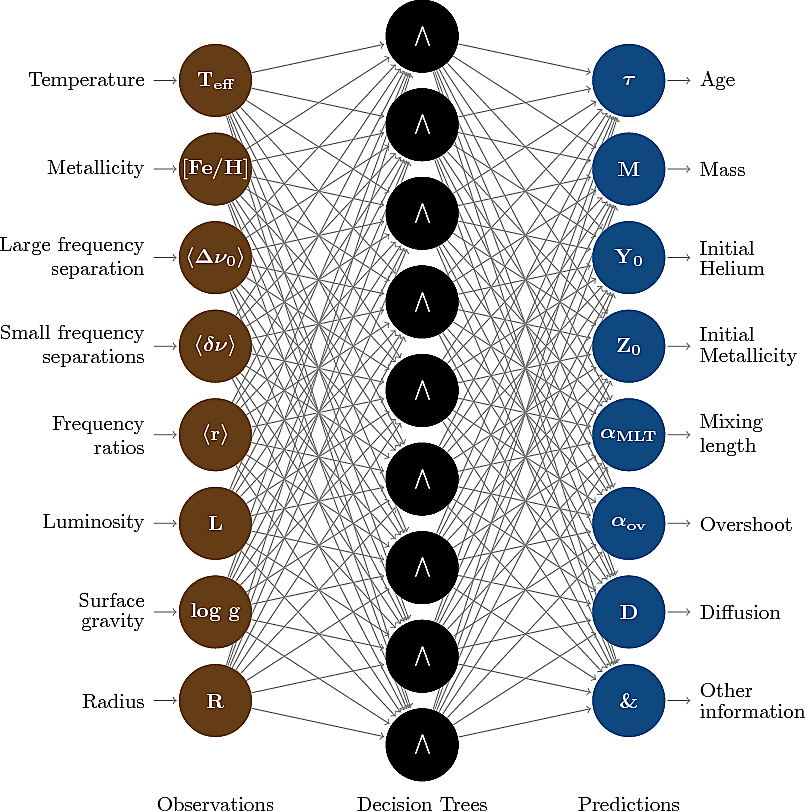
\includegraphics{figs/random_forest.pdf}
    \caption{A schematic representation of a random forest regressor for inferring fundamental stellar parameters. Classical observables such as temperature and global asteroseismic observables like $\langle\delta\nu_{0,2}\rangle$ are input on the left side. These quantities are then fed through to some number of hidden decision trees, which each independently predict attributes like age and mass. The predictions are then averaged and output on the right side. All inputs and outputs are optional. For example, surface gravities, luminosities, and radii are not always available (e.g.\ with the KOI stars). In their absence, these quantities can be predicted instead of being supplied. In this case, those nodes can be moved over to the ``prediction'' side instead of being on the ``observations'' side. Also, in addition to potentially unobserved inputs like stellar radii, other interesting model properties can be predicted as well, such as core hydrogen mass fraction and surface helium. \label{fig:rf} }
\end{figure*}


\subsubsection{Feature Importances}
\label{sec:importances}
A random forest is an ensemble regressor, meaning that it is composed of many individual components that each perform statistical regression, and the forest subsequently averages over the results from each component \citep{breiman2001random}. The components of the ensemble are decision trees, each of which learns a set of decision rules for relating the observations to the model parameters. Each decision tree is given a random subset of the evolutionary models and a random subset of the observable quantities, a process known as statistical bagging \citep[][Section 8.7]{hastie2005elements}, which prevents the random forest from over-fitting the training data. 

The decision trees use information theory to decide which rule is the best choice for inferring quantities like age and mass from the supplied information \citep[][Chapter 9]{hastie2005elements}. At every stage, the rule that creates the largest decrease in mean squared error (MSE) is crafted. A rule may be, for example, ``all models with L $<0.4$ L$_\odot$ have M $<$ M$_\odot$.'' Rules are created until every data point that was supplied to that particular tree is fully explained by a sequence of decisions. We moreover use a variant on random forests known as \emph{extremely} randomized trees \citep{geurts2006extremely}, which further randomizes the attribute splittings and the location of the cut-point used when creating decision rules. 

This process presents an opportunity for not only inferring stellar parameters from observations, but also for understanding the relationships that exist in the simulations. This is because each decision tree explicitly ranks the relative ``importance'' of each observable quantity, where importance is defined in terms of the reduction in MSE after defining a decision rule based on that attribute. Figure \ref{fig:importances} shows the distributions of relative importances over all of the trees in the forest for each type of observation in inferring stellar parameters. The attributes that are used most often to construct decision rules are metallicity and temperature, which are each significantly more important attributes than the rest in resolving stellar parameters. The importance of [Fe/H] is due to the fact that the determinations of quantities like the Z$_0$ and D depend nearly entirely on it. Figure \ref{fig:importance-covariances} furthermore shows the covariances of these importances, which demonstrates which combinations of variables are most useful for constraining stellar parameters. For example, this diagram shows that in the decision trees where [Fe/H] is most useful in creating decision rules, knowledge of stellar radii is deemed to be less important. Note that importance does not indicate indispensability: an appreciable fraction of decision rules being made based off of an observable quantity does not mean that another forest without that quantity would not perform just as well. That being said, these results indicate that the best area to improve measurements would be in metallicity determinations, because for stars being predicted using this random forest, less precise values here means exploring many more paths and hence arriving at less certain predictions. %as we will see, several of these attributes can be removed without affecting the quality of predictions. 
%regions of the parameter space where [Fe/H] is most useful in constraining stellar parameters correspond to a relative lack of usefulness in other parameters such as radii or surface gravities. 
%It reveals, for example, that regions of the parameter space that are best divided by knowledge of [Fe/H] are significantly less divisible by knowledge of attributes like the radius. %that constructing a rule based on [Fe/H] makes knowledge of other surface attributes such as the radius or surface gravity less important for constraining stellar attributes. 
%For example, the redness of the top left cell between the asteroseismic frequency ratio $\langle r_{1,3} \rangle$ (abscissa) and the surface gravity log g (ordinate) indicates that while this ratio is the most useful quantity for making inferences, a tree will often supplement it with information about the surface---which by construction the ratios lack---to complete an analysis. Likewise, the large covariance between T$_{\text{eff}}$ and [Fe/H] is due to the fact that the effective temperature of a star is not only a function of its mass but also its composition.%Taken together, these two plots illustrate what combination of variables provide the best connections for determining stellar parameters. 

\begin{figure}
    \centering
    \includegraphics[width=\colwidth, keepaspectratio]{figs/importances/importances-perturb.pdf}
    \caption{Relative importances for each observable feature in inferring fundamental stellar parameters as measured by a random forest regressor grown from a grid of evolutionary models. The boxes display the first (16\%) and third (84\%) quartile of feature importances over all trees, the middle line indicates the median, and the whiskers extend to the most extreme values. The boxes are sorted by the median value.}
    \label{fig:importances}
\end{figure}

\begin{figure*}
    \centering
    \includegraphics[width=\linewidth, keepaspectratio]{figs/importances/cov-perturb.pdf}
    \caption{Standardized covariances of random forest feature importances with variables shown in order of median importance. Larger values of the covariance indicates that the parameters are often used together, whereas smaller values indicate redundancy. } 
    \label{fig:importance-covariances}
\end{figure*}

For many stars, information such as radii, luminosities, surface gravities, and/or oscillation modes with spherical degree $\ell=3$ are not available from observations. For example, the KOI data set lacks all of this information, and the hare-and-hound exercise data lack all of these except luminosities. We therefore must train random forests that predict those quantities instead of using them as inputs. We show the relative importances determined by these forests in Figure \ref{fig:importances2}. When $\ell=3$ modes and luminosities are omitted, effective temperatures jump in importance and tie with [Fe/H] as the most important quantity to have observed. 

\begin{figure*}
    \centering
    \includegraphics[width=0.5\linewidth,keepaspectratio]{figs/importances/importances-hares.pdf}\hfill
    \includegraphics[width=0.5\linewidth, keepaspectratio]{figs/importances/importances-kages.pdf}
    \caption{Box-and-whisker plots of relative importances for each observable feature in measuring fundamental stellar parameters for the hare-and-hound exercise data (left), where luminosities are available; and the Kepler objects-of-interest (right), where they are not. Octupole ($\ell=3$) modes have not been measured in any of these stars, so $\langle\delta\nu_{1,3}\rangle$ and $\langle r_{1,3}\rangle$ from evolutionary modelling are not supplied to these random forests. \label{fig:importances2} }
\end{figure*}


\subsubsection{Uncertainty}
\label{sec:uncertainties}
There are three separate sources of uncertainty in predicting stellar parameters. The first is the systematic uncertainty in the physics used to model stars. These uncertainties are unknown, however, and hence cannot be propagated. The second is the uncertainty belonging to the observations of the star. We propagate measurement uncertainties $\sigma$ into the predictions by perturbing all measured quantities $n=10,000$ times with normal noise having zero mean and standard deviation $\sigma$. We account for the covariance between asteroseismic separations and ratios by recalculating them upon each perturbation. 

The final source is model uncertainty. Fundamentally, each parameter can only be constrained to the extent that observations are able to bear information pertaining to that parameter. Even if observations were error-free, there still may exist a limit to which information gleaned from the surface may tell us about the physical attributes and evolutionary history of a star. We quantify those limits via cross-validation: we train the random forest on only a subset of the simulated evolutionary tracks and make predictions on a held-out validation set. We randomly select a different subset of the tracks 25 times to serve as different held-out validation sets and obtain averaged accuracy scores. 

We calculate accuracies using several scores. The first is the explained variance score V$_{\text{e}}$:
\begin{equation}
  \text{V}_{\text{e}} = 1 - \frac{\text{Var}\{ y - \hat y \}}{\text{Var}\{ y \}}
\end{equation}
where $y$ is the value we want to predict from the validation set (e.g.\ stellar mass), $\hat y$ is the predicted value from the random forest, and Var is the variance, i.e.\ the square of the standard deviation. This score tells us the extent to which the regressor has reduced the variance in the parameter it is predicting. The value ranges from negative infinity, which would be obtained by a pathologically bad predictor; to one for a perfect predictor, which occurs if all of the values are predicted with zero error. 

The next score we consider is the residuals of each prediction, i.e.\ the absolute difference between the true value $y$ and the predicted value $\hat y$. Naturally we want this value to be as low as possible. We also consider the precision of the model $\hat \sigma$ by taking the standard deviation of predictions across all of the decision trees in the forest. Finally, we consider these scores together by calculating the distance of the residuals in units of model precision, i.e.\ $\abs{\hat y - y} / \hat{\sigma}$. 

Figure \ref{fig:evaluation-tracks} shows these accuracies as a function of the number of evolutionary tracks used in the training of the random forest. Since the residuals and standard deviations of each parameter are incomparable, we normalize them using the usual definition, i.e.\
\begin{equation}
  \tilde p \equiv \frac{p - \max(p)}{\max(p)-\min(p)}
\end{equation}
where $p$ is any parameter (e.g.\ stellar mass). We also consider the number of trees in the forest and the number of models per evolutionary track; see Appendix \ref{sec:evaluation} for an extended discussion.

\begin{figure*}
    \centering
    \includegraphics[width=0.5\linewidth,keepaspectratio]{figs/evaluation/legend.png}\\
    \includegraphics[width=0.5\linewidth,keepaspectratio]{figs/evaluation/num_tracks-ev.pdf}\hfill
    \includegraphics[width=0.5\linewidth,keepaspectratio]{figs/evaluation/num_tracks-dist.pdf}\\
    \includegraphics[width=0.5\linewidth,keepaspectratio]{figs/evaluation/num_tracks-diff.pdf}\hfill
    \includegraphics[width=0.5\linewidth,keepaspectratio]{figs/evaluation/num_tracks-sigma.pdf}\\
    \caption{Evaluations of model accuracy. Explained variance (top left), accuracy per precision distance (top right), normalized absolute error (bottom left), and normalized model uncertainty (bottom right) for each stellar parameter as a function of the number of evolutionary tracks used in training the random forest. } 
    \label{fig:evaluation-tracks}
\end{figure*}

When supplied with enough simulations, the random forest reduces the variance in each parameter and is able to make precise inferences. Indeed, most attributes have very little model uncertainty when being inferred by a well-trained random forest. For example, essentially all of the uncertainty in predicting stellar radii and luminosities will stem from observational error. However, for some model properties---most notably the mixing length parameter---there is still a great deal of model uncertainty. Prior to about 500 evolutionary tracks, the difference between the absolute and predicted mixing lengths actually have a greater variance than the raw mixing lengths themselves. Likewise, the diffusion factor is difficult to constrain because a star can achieve the same present-day [Fe/H] by having a large initial non-hydrogen abundance and a large diffusion factor as it can by having the same initial [Fe/H] but with no diffusion. These difficult-to-constrain attributes will therefore be predicted with substantial error bars regardless of the precision of the observations. 

%On the other hand, the accuracy per precision score shows that the regressor is well-calibrated: in the average case, the values are predicted within one $\hat\sigma$ as desired. In other words, the uncertainties for all of the parameters---even for the ones that cannot be constrained very well---are still appropriately gauged by the regressor. 


%%%%%%%%%%%%%%%%%%%%%%%%%%%%%%%%%%%%%%%%%
%%% Results %%%%%%%%%%%%%%%%%%%%%%%%%%%%%
%%%%%%%%%%%%%%%%%%%%%%%%%%%%%%%%%%%%%%%%%
\section{Results}
We perform three tests of our method. We begin with a hare-and-hound simulation exercise to show that we can can reliably recover parameters with known truth values. We then move to the Sun and the solar-like stars 16 Cyg A \& B, which have been the subjects of many investigations; and we conclude by applying our method to 33 Kepler objects-of-interest. In each case, we train our random forest regressor on the subset of observational data that is available to the stars being processed. In the case of the Sun and 16 Cygni, we know very accurately their radii, luminosities, and surface gravities. For other stars, however, we predict this information rather than supplying it as an input. 


%%%%%%%%%%%%%%%%%%%%%%%%%%%%%%%%%%%%%%%%%
%%% Hare and Hound %%%%%%%%%%%%%%%%%%%%%%
%%%%%%%%%%%%%%%%%%%%%%%%%%%%%%%%%%%%%%%%%
\subsection{Hare and Hound} 
We performed a blind hare-and-hound exercise to evaluate the performance of our predictor. Author S.B.\ prepared twelve models varied in mass, initial chemical composition, and mixing length parameter with only some models having overshooting and only some models having atomic diffusion included. The models were evolved without rotation using the Yale rotating stellar evolution code \citep[YREC;][]{2008Ap&SS.316...31D}, which is a different evolution code than the one that was used to train the random forest. Effective temperatures, luminosities, [Fe/H] and $\nu_{\max}$ values as well as $\ell=0,1,2$ frequencies were obtained from each model. Author G.C.A.\  perturbed the ``observations'' of these models according to the scheme devised by \citet{spaceinn}. The true values and the perturbed observations can be seen in Appendix \ref{sec:hare-and-hound}. The perturbed observations and their uncertainties were given to author E.P.B.\@, who used the machine learning methods described herein to recover the stellar parameters of the models without being given access to the true values. The predicted ages, masses, and radii for these models are plotted against their true values in Figure \ref{fig:hare-comparison}. The method is able to recover the true model values within uncertainties even when they have been perturbed by noise. We do not compare the predicted mixing length parameter, overshooting parameter or diffusion factor because they depend on the physics of the evolutionary code used, e.g.\ the choice in stellar atmosphere. 

\begin{figure}
    \centering
    \includegraphics[width=\colwidth,keepaspectratio]{figs/comparison/basu-Age-rel.pdf}\\
    \includegraphics[width=\colwidth,keepaspectratio]{figs/comparison/basu-Mass-rel.pdf}\\
    \includegraphics[width=\colwidth,keepaspectratio]{figs/comparison/basu-Radius-rel.pdf}
    \caption{Relative differences between the predicted and true values for age, mass, and radius as a function of the true values in a hare-and-hound simulation exercise.%Predicted values of age, mass, and radius plotted against the true values in a hare-and-hound simulation exercise. 
    \label{fig:hare-comparison}}
\end{figure}


%%%%%%%%%%%%%%%%%%%%%%%%%%%%%%%%%%%%%%%%%
%%% The Sun & 16 Cygni %%%%%%%%%%%%%%%%%%
%%%%%%%%%%%%%%%%%%%%%%%%%%%%%%%%%%%%%%%%%
\subsection{The Sun and 16 Cygni}
To ensure confidence in our predictions on Kepler data, we first degrade the frequencies of the Sun at solar minimum that were obtained by the Birmingham Solar-Oscillations Network \citep[BiSON;][]{2014MNRAS.439.2025D} to the level of information that is achievable by the spacecraft. We also degrade the Sun's uncertainties of classical observations by applying 16 Cyg B's uncertainties of effective temperature, luminosity, surface gravity, metallicity, $\nu_{\max}$, radius, and radial velocity. Finally, we perturb each value with random Gaussian noise according to its uncertainty to reflect the fact that the measured value of an uncertain observation is not \emph{per se} the true value. We show in Figure \ref{fig:corner} the densities for the predicted mass, initial composition, mixing length parameter, overshoot coefficient, and diffusion factor needed for fitting an evolutionary model to degraded data of the Sun, and also the predicted age, core hydrogen abundance, and surface helium abundance of the Sun. Relative uncertainties $\epsilon=100\cdot\sigma/\mu$ are also indicated, where $\mu$ is the mean and $\sigma$ is the standard deviation. Several parameters show multimodality due to model degeneracies. For example, two solutions for the initial helium are present because it covaries with the mixing length parameter: the higher peak of Y$_0$ corresponds to the lower peak of $\alpha_{\text{MLT}}$ and vice versa. Likewise, high values of surface helium correspond to low values of the diffusion factor. 

\begin{figure*}
    \centering
    \includegraphics[width=\linewidth,keepaspectratio]{figs/comparison/Tagesstern.pdf}
    \caption{Predictions from machine learning of initial (top six) and current-age (bottom three) stellar parameters for degraded solar data. Labels are placed at the mean and 3$\sigma$ levels. Dotted lines indicate the median and quartiles. Relative uncertainties $\epsilon$ are shown beside each plot. Note that the overshoot parameter applies to all convective boundaries and is not modified over the course of evolution, so its non-zero value does not imply that the Sun has a convective core. } 
    \label{fig:corner}
\end{figure*}

Effective temperatures, surface gravities, and metallicities of 16 Cyg A and B were obtained from \citet{2009A&A...508L..17R}; radii and luminosities from \citet{2013MNRAS.433.1262W}; and frequencies from \citet{2015MNRAS.446.2959D}. We obtained the radial velocity measurements of 16 Cyg A and B from \citet{2002ApJS..141..503N} and corrected frequencies for Doppler shifting as per the prescription in \citet{2014MNRAS.445L..94D}. We tried with and without line-of-sight corrections and found that it did not affect the predicted quantities or their uncertainties. We used a random forest trained on effective temperatures, metallicities, luminosities, surface gravities, radii, and global asteroseismic observables $\langle \Delta\nu_0 \rangle$, $\langle \delta\nu_{0,2} \rangle$, $\langle \delta\nu_{1,3} \rangle$, $\langle r_{0,2} \rangle$, $\langle r_{1,3} \rangle$, $\langle r_{0,1} \rangle$, and $\langle r_{1,0} \rangle$ to predict the properties of these stars. The initial parameters---masses, chemical compositions, mixing lengths, diffusion factors, and overshoot coefficients---for 16 Cygni as predicted by machine learning can be seen in Table \ref{tab:results}, and the predicted current parameters---age, surface helium and core hydrogen abundances---can be seen in Table \ref{tab:results-ca}. For reference we also show there the predicted solar values from these inputs as well. These results support the hypothesis that 16 Cyg A and B were co-natal; i.e.\ they formed at the same time with the same initial composition. 


\begin{deluxetable*}{cccccccc}
\tabletypesize{\scriptsize}
\tablecaption{Means and standard deviations for initial stellar parameters of 16 Cyg A and B as inferred by machine learning. The values obtained from degraded solar data predicted on these quantities are shown for reference.
\label{tab:results}}
\tablewidth{0pt}
\tablehead{\colhead{Name} & \colhead{M$/$M$_\odot$} & \colhead{Y$_0$} & \colhead{Z$_0$} & \colhead{$\alpha_{\mathrm{MLT}}$} & \colhead{$\alpha_{\mathrm{ov}}$} & \colhead{D}}
\startdata
16 Cyg A & 1.08 $\pm$ 0.016 & 0.262 $\pm$ 0.0073 & 0.022 $\pm$ 0.0014 & 1.86 $\pm$ 0.077 & 0.07 $\pm$ 0.028 & 0.9 $\pm$ 0.76 \\
16 Cyg B & 1.03 $\pm$ 0.015 & 0.268 $\pm$ 0.0065 & 0.021 $\pm$ 0.0015 & 1.83 $\pm$ 0.069 & 0.11 $\pm$ 0.029 & 1.9 $\pm$ 1.57 \\
Sun      & 1.00 $\pm$ 0.012 & 0.270 $\pm$ 0.0062 & 0.020 $\pm$ 0.0014 & 1.88 $\pm$ 0.078 & 0.06 $\pm$ 0.015 & 3.7 $\pm$ 3.18
\enddata
\end{deluxetable*}


\begin{deluxetable*}{cccc}
\tabletypesize{\scriptsize}
\tablecaption{Means and standard deviations for current-age stellar attributes of 16 Cyg A and B as inferred by machine learning. The values obtained from degraded solar data predicted on these quantities are shown for reference. \label{tab:results-ca}}
\tablewidth{0pt}
\tablehead{\colhead{Name} & \colhead{$\tau/$Gyr} & \colhead{X$_{\mathrm{c}}$} & \colhead{Y$_{\mathrm{surf}}$}}
\startdata
16 Cyg A & 6.9 $\pm$ 0.40 & 0.06 $\pm$ 0.024 & 0.246 $\pm$ 0.0085 \\
16 Cyg B & 6.8 $\pm$ 0.28 & 0.15 $\pm$ 0.023 & 0.24  $\pm$ 0.017 \\
Sun      & 4.6 $\pm$ 0.20 & 0.34 $\pm$ 0.027 & 0.24  $\pm$ 0.017
\enddata
\end{deluxetable*}

We additionally predict the radii and luminosities of 16 Cyg A and B instead of using them as constraints. Figure \ref{fig:interferometry} shows our inferred radii, luminosities and surface helium abundances of 16 Cyg A and B plotted against the values determined by interferometry \citep{2013MNRAS.433.1262W} and an asteroseismic estimate \citep{2014ApJ...790..138V}. Here again we find excellent agreement between our method and the measured values. 

\begin{figure*}
    \centering
    \includegraphics[width=0.5\linewidth, keepaspectratio]{figs/hists/cyg-radius.pdf}\hfill
    \includegraphics[width=0.5\linewidth, keepaspectratio]{figs/hists/cyg-L.pdf}\\
    \includegraphics[width=0.5\linewidth, keepaspectratio]{figs/hists/cyg-Y_surf.pdf}
    \caption{Probability densities for predictions of 16 Cyg A (red) and B (blue) from machine learning of radii (top), luminosities (middle), and surface helium abundances (bottom). Relative uncertainties $\epsilon$ are shown beside each plot. Predictions and $2\sigma$ uncertainties from interferometric (``int'') measurements and asteroseismic (``ast'') estimates are shown with arrows.}
    \label{fig:interferometry}
\end{figure*}

\citet{2015ApJ...811L..37M} performed detailed modelling of 16 Cyg A and B using the Asteroseismic Modeling Portal (AMP), a genetic algorithm for matching individual frequencies of stars to stellar models. They calculated their results using without heavy element diffusion (i.e.\ only helium diffusion), without overshooting, and with a fixed diffusion factor. In order to account for systematic uncertainties, they multiplied the spectroscopic uncertainties of 16 Cyg A and B by an arbitrary constant $C=3$. Therefore, in order to make a fair comparison between the results of our method and theirs, we generate a new matrix of evolutionary models with those same conditions and also increase the uncertainties on [Fe/H] by a factor of $C$. In Figure \ref{fig:16Cyg-hist}, we show probability densities of the predicted parameters of 16 Cyg A and B that we obtain using machine learning in comparison with the results obtained by AMP. We find the values and uncertainties agree well. To perform their analysis, AMP required more than 15,000 hours of CPU time to model 16 Cyg A and B using the world's 10th fastest supercomputer, the Texas Advanced Computing Center Stampede \citep{TOP500}. Here we have obtained comparable results in less than one minute using only global asteroseismic constraints and no individual frequencies. Although more computationally expensive than our method, detailed optimization codes do have advantages in that they are able to obtain detailed structural models of the stars as well as characterize stars beyond the main-sequence, where our method has not yet been extended. 
%We note however that detailed optimization codes like AMP remain important for obtaining structural models of stars as well as for performing post-main sequence modelling, where our method has not yet been extended. 

\begin{figure*}
    \centering
    \includegraphics[width=0.5\linewidth, keepaspectratio]{figs/hists/cyg-age.pdf}\hfill
    \includegraphics[width=0.5\linewidth, keepaspectratio]{figs/hists/cyg-M.pdf}\\
    \includegraphics[width=0.5\linewidth, keepaspectratio]{figs/hists/cyg-Y.pdf}\hfill
    \includegraphics[width=0.5\linewidth, keepaspectratio]{figs/hists/cyg-Z.pdf}
    \caption{Probability densities showing predictions from machine learning of fundamental stellar parameters for 16 Cyg A (red) and B (blue) against predictions from AMP modelling. Relative uncertainties are shown beside each plot. Predictions and $2\sigma$ uncertainties from AMP modelling are shown with arrows.}
    \label{fig:16Cyg-hist}
\end{figure*}


%%%%%%%%%%%%%%%%%%%%%%%%%%%%%%%%%%%%%%%%%
%%% Kepler Objects of Interest %%%%%%%%%%
%%%%%%%%%%%%%%%%%%%%%%%%%%%%%%%%%%%%%%%%%
\subsection{Kepler Objects of Interest}
We obtain classical observations and frequencies of the KOI targets from \citet[hereinafter KAGES]{2015MNRAS.452.2127S}. We use line-of-sight radial velocity corrections when available, which was only the case with KIC 6278762 \citep{2002AJ....124.1144L}, KIC 10666592 \citep{2013A&A...554A..84M}, and KIC 3632418 \citep{2006AstL...32..759G}. We use the random forest whose feature importances were shown in Figure \ref{fig:importances2} to predict the fundamental properties of these stars; that is, the random forest that is trained on effective temperatures, metallicities, and global asteroseismic observables $\langle \Delta\nu_0 \rangle$, $\langle \delta\nu_{0,2} \rangle$, $\langle r_{0,2} \rangle$, $\langle r_{0,1} \rangle$, and $\langle r_{1,0} \rangle$. The predicted initial conditions---masses, chemical compositions, mixing lengths, overshoot coefficients, and diffusion factors---can be seen in Table \ref{tab:results-kages}; and the predicted current conditions---ages, core hydrogen abundances, surface gravities, luminosities, radii, and surface helium abundances---can be seen in Table \ref{tab:results-kages-curr}. Figure \ref{fig:us-vs-them} shows the fundamental parameters obtained from our method plotted against those obtained by KAGES. We find good agreement across all stars. Although still in statistical agreement, the median values of our predicted ages are systematically younger and the median values of our predicted masses are systematically heavier than those predicted by KAGES. 
 Without direct access to their models, the exact reason is difficult to pinpoint but given the differences in the choice of input physics the results are perhaps not so surprising. 
 %we expect that differences in the choice of input physics is a key factor.  %This is because we consider overshooting calculations in our models, which, with all else being equal, results in stars having larger core masses and therefore being more evolved at the same age. 
We vary the efficiency of diffusion, the extent of core overshoot and the value of the mixing length parameter, whereas their models are calculated with or without a constant value of diffusion, without core overshoot and with a solar calibrated mixing length efficiency.   


We find a significant linear trend in the Kepler objects-of-interest between the diffusion factor and stellar mass needed to reproduce observations ($P = 0.0001$ from a two-sided t-test with $N-2=31$ degrees of freedom). Since the values of mass and diffusion factor are uncertain, we use Deming regression to estimate the coefficients of this relation without regression dilution \citep{deming1943statistical}. We show the fitted diffusion factors as a function of predicted stellar mass for all of these stars in Figure \ref{fig:diffusion}. We find that a diffusion factor linearly decreasing with mass, i.e.\ 
\begin{equation} \label{eq:diffusion}
    \text{D} = ( 8.6 \pm 1.94 ) - ( 5.6 \pm 1.37 ) \cdot \text{M}/\text{M}_\odot
\end{equation}
explains observations better than any constant diffusion factor (e.g.\ D=1 or D=0). 

\begin{deluxetable*}{ccccccc}
\tabletypesize{\scriptsize}
\tablecaption{Means and standard deviations for initial conditions of the KOI data set inferred via machine learning. The values obtained from degraded solar data predicted on these quantities are shown for reference. \label{tab:results-kages}}
\tablewidth{0pt}
\tablehead{\colhead{KIC} & \colhead{M$/$M$_\odot$} & \colhead{Y$_0$} & \colhead{Z$_0$} & \colhead{$\alpha_{\mathrm{MLT}}$} & \colhead{$\alpha_{\mathrm{ov}}$} & \colhead{D}}
\startdata
 3425851 & 1.15 $\pm$ 0.053  & 0.28  $\pm$ 0.020  & 0.015 $\pm$ 0.0028 & 1.9  $\pm$ 0.23  & 0.06 $\pm$ 0.057 &  0.5 $\pm$  0.92 \\
 3544595 & 0.91 $\pm$ 0.032  & 0.270 $\pm$ 0.0090 & 0.015 $\pm$ 0.0028 & 1.9  $\pm$ 0.10  & 0.2  $\pm$ 0.11  &  4.9 $\pm$  4.38 \\
 3632418 & 1.39 $\pm$ 0.057  & 0.267 $\pm$ 0.0089 & 0.019 $\pm$ 0.0032 & 2.0  $\pm$ 0.12  & 0.2  $\pm$ 0.14  &  1.1 $\pm$  1.01 \\
 4141376 & 1.03 $\pm$ 0.036  & 0.267 $\pm$ 0.0097 & 0.012 $\pm$ 0.0025 & 1.9  $\pm$ 0.12  & 0.1  $\pm$ 0.11  &  4.0 $\pm$  4.09 \\
 4143755 & 0.99 $\pm$ 0.037  & 0.277 $\pm$ 0.0050 & 0.014 $\pm$ 0.0026 & 1.77 $\pm$ 0.033 & 0.37 $\pm$ 0.071 & 13.4 $\pm$  5.37 \\
 4349452 & 1.22 $\pm$ 0.056  & 0.28  $\pm$ 0.012  & 0.020 $\pm$ 0.0043 & 1.9  $\pm$ 0.17  & 0.10 $\pm$ 0.090 &  7.3 $\pm$  8.82 \\
 4914423 & 1.19 $\pm$ 0.048  & 0.274 $\pm$ 0.0097 & 0.026 $\pm$ 0.0046 & 1.8  $\pm$ 0.11  & 0.08 $\pm$ 0.043 &  2.3 $\pm$  1.6 \\
 5094751 & 1.11 $\pm$ 0.038  & 0.274 $\pm$ 0.0082 & 0.018 $\pm$ 0.0030 & 1.8  $\pm$ 0.11  & 0.07 $\pm$ 0.041 &  2.3 $\pm$  1.39 \\
 5866724 & 1.29 $\pm$ 0.065  & 0.28  $\pm$ 0.011  & 0.027 $\pm$ 0.0058 & 1.8  $\pm$ 0.13  & 0.12 $\pm$ 0.086 &  7.0 $\pm$  8.38 \\
 6196457 & 1.31 $\pm$ 0.058  & 0.276 $\pm$ 0.005  & 0.032 $\pm$ 0.0050 & 1.71 $\pm$ 0.050 & 0.16 $\pm$ 0.055 &  5.7 $\pm$  2.34 \\
 6278762 & 0.76 $\pm$ 0.012  & 0.254 $\pm$ 0.0058 & 0.013 $\pm$ 0.0017 & 2.09 $\pm$ 0.069 & 0.06 $\pm$ 0.028 &  5.3 $\pm$  2.23 \\
 6521045 & 1.19 $\pm$ 0.046  & 0.273 $\pm$ 0.0071 & 0.027 $\pm$ 0.0044 & 1.82 $\pm$ 0.074 & 0.12 $\pm$ 0.036 &  3.2 $\pm$  1.31 \\
 7670943 & 1.30 $\pm$ 0.061  & 0.28  $\pm$ 0.017  & 0.021 $\pm$ 0.0045 & 2.0  $\pm$ 0.23  & 0.06 $\pm$ 0.064 &  1.0 $\pm$  2.55 \\
 8077137 & 1.23 $\pm$ 0.070  & 0.270 $\pm$ 0.0093 & 0.018 $\pm$ 0.0028 & 1.8  $\pm$ 0.14  & 0.2  $\pm$ 0.11  &  2.9 $\pm$  2.08 \\
 8292840 & 1.15 $\pm$ 0.079  & 0.28  $\pm$ 0.010  & 0.016 $\pm$ 0.0049 & 1.8  $\pm$ 0.15  & 0.1  $\pm$ 0.12  & 11.  $\pm$ 10.7  \\
 8349582 & 1.23 $\pm$ 0.040  & 0.271 $\pm$ 0.0069 & 0.043 $\pm$ 0.0074 & 1.9  $\pm$ 0.12  & 0.11 $\pm$ 0.060 &  2.5 $\pm$  1.11 \\
 8478994 & 0.81 $\pm$ 0.022  & 0.272 $\pm$ 0.0082 & 0.010 $\pm$ 0.0012 & 1.91 $\pm$ 0.054 & 0.21 $\pm$ 0.068 & 17.  $\pm$  9.74 \\
 8494142 & 1.42 $\pm$ 0.058  & 0.27  $\pm$ 0.010  & 0.028 $\pm$ 0.0046 & 1.70 $\pm$ 0.064 & 0.10 $\pm$ 0.051 &  1.6 $\pm$  1.65 \\
 8554498 & 1.39 $\pm$ 0.067  & 0.272 $\pm$ 0.0082 & 0.031 $\pm$ 0.0032 & 1.70 $\pm$ 0.077 & 0.14 $\pm$ 0.079 &  1.7 $\pm$  1.17 \\
 8684730 & 1.44 $\pm$ 0.030  & 0.277 $\pm$ 0.0075 & 0.041 $\pm$ 0.0049 & 1.9  $\pm$ 0.14  & 0.29 $\pm$ 0.094 & 15.2 $\pm$  8.81 \\
 8866102 & 1.26 $\pm$ 0.069  & 0.28  $\pm$ 0.013  & 0.021 $\pm$ 0.0048 & 1.8  $\pm$ 0.15  & 0.08 $\pm$ 0.070 &  5.  $\pm$  7.48 \\
 9414417 & 1.36 $\pm$ 0.054  & 0.264 $\pm$ 0.0073 & 0.018 $\pm$ 0.0028 & 1.9  $\pm$ 0.13  & 0.2  $\pm$ 0.1   &  2.2 $\pm$  1.68 \\
 9592705 & 1.45 $\pm$ 0.038  & 0.27  $\pm$ 0.010  & 0.029 $\pm$ 0.0038 & 1.72 $\pm$ 0.064 & 0.12 $\pm$ 0.056 &  0.6 $\pm$  0.47 \\
 9955598 & 0.93 $\pm$ 0.028  & 0.27  $\pm$ 0.011  & 0.023 $\pm$ 0.0039 & 1.9  $\pm$ 0.10  & 0.2  $\pm$ 0.13  &  2.2 $\pm$  1.76 \\
10514430 & 1.13 $\pm$ 0.053  & 0.277 $\pm$ 0.0046 & 0.021 $\pm$ 0.0039 & 1.78 $\pm$ 0.059 & 0.30 $\pm$ 0.097 &  4.7 $\pm$  1.77 \\
10586004 & 1.31 $\pm$ 0.078  & 0.274 $\pm$ 0.0055 & 0.038 $\pm$ 0.0071 & 1.8  $\pm$ 0.13  & 0.2  $\pm$ 0.13  &  4.3 $\pm$  3.99 \\
10666592 & 1.50 $\pm$ 0.023  & 0.30  $\pm$ 0.013  & 0.030 $\pm$ 0.0032 & 1.8  $\pm$ 0.11  & 0.06 $\pm$ 0.043 &  0.2 $\pm$  0.14 \\
10963065 & 1.09 $\pm$ 0.031  & 0.264 $\pm$ 0.0083 & 0.014 $\pm$ 0.0025 & 1.8  $\pm$ 0.11  & 0.05 $\pm$ 0.027 &  3.1 $\pm$  2.68 \\
11133306 & 1.11 $\pm$ 0.044  & 0.272 $\pm$ 0.0099 & 0.021 $\pm$ 0.0040 & 1.8  $\pm$ 0.16  & 0.04 $\pm$ 0.033 &  5.  $\pm$  5.75 \\
11295426 & 1.11 $\pm$ 0.033  & 0.27  $\pm$ 0.010  & 0.025 $\pm$ 0.0036 & 1.81 $\pm$ 0.084 & 0.05 $\pm$ 0.035 &  1.3 $\pm$  0.87 \\
11401755 & 1.15 $\pm$ 0.039  & 0.271 $\pm$ 0.0057 & 0.015 $\pm$ 0.0023 & 1.88 $\pm$ 0.055 & 0.33 $\pm$ 0.071 &  3.8 $\pm$  1.81 \\
11807274 & 1.32 $\pm$ 0.079  & 0.276 $\pm$ 0.0097 & 0.024 $\pm$ 0.0051 & 1.77 $\pm$ 0.083 & 0.11 $\pm$ 0.066 &  5.4 $\pm$  5.61 \\
11853905 & 1.22 $\pm$ 0.055  & 0.272 $\pm$ 0.0072 & 0.029 $\pm$ 0.0050 & 1.8  $\pm$ 0.12  & 0.18 $\pm$ 0.086 &  3.3 $\pm$  1.85 \\
11904151 & 0.93 $\pm$ 0.033  & 0.265 $\pm$ 0.0091 & 0.016 $\pm$ 0.0030 & 1.8  $\pm$ 0.13  & 0.05 $\pm$ 0.029 &  3.1 $\pm$  2.09 \\
     Sun & 1.00 $\pm$ 0.0093 & 0.266 $\pm$ 0.0035 & 0.018 $\pm$ 0.0011 & 1.81 $\pm$ 0.032 & 0.07 $\pm$ 0.021 &  2.1 $\pm$  0.83
\enddata
\end{deluxetable*}

\begin{deluxetable*}{ccccccc}
\tabletypesize{\scriptsize}
\tablecaption{Means and standard deviations for current-age conditions of the KOI data set inferred via machine learning. The values obtained from degraded solar data predicted on these quantities are shown for reference. \label{tab:results-kages-curr}}
\tablewidth{0pt}
\tablehead{\colhead{KIC} & \colhead{$\tau/$Gyr} & \colhead{X$_{\mathrm{c}}$} & \colhead{log g} & \colhead{L$/$L$_\odot$} & \colhead{R$/$R$_\odot$} & \colhead{Y$_{\mathrm{surf}}$}}
\startdata
 3425851 &  3.7 $\pm$ 0.76  & 0.14  $\pm$ 0.081  & 4.234 $\pm$ 0.0098 & 2.7  $\pm$ 0.16  & 1.36  $\pm$ 0.022  & 0.27  $\pm$ 0.026 \\
 3544595 &  6.7 $\pm$ 1.47  & 0.31  $\pm$ 0.078  & 4.46  $\pm$ 0.016  & 0.84 $\pm$ 0.068 & 0.94  $\pm$ 0.020  & 0.23  $\pm$ 0.023 \\
 3632418 &  3.0 $\pm$ 0.36  & 0.10  $\pm$ 0.039  & 4.020 $\pm$ 0.0076 & 5.2  $\pm$ 0.25  & 1.91  $\pm$ 0.031  & 0.24  $\pm$ 0.021 \\
 4141376 &  3.4 $\pm$ 0.67  & 0.38  $\pm$ 0.070  & 4.41  $\pm$ 0.011  & 1.42 $\pm$ 0.097 & 1.05  $\pm$ 0.019  & 0.24  $\pm$ 0.022 \\
 4143755 &  8.0 $\pm$ 0.80  & 0.07  $\pm$ 0.022  & 4.09  $\pm$ 0.013  & 2.3  $\pm$ 0.12  & 1.50  $\pm$ 0.029  & 0.17  $\pm$ 0.023 \\
 4349452 &  2.4 $\pm$ 0.78  & 0.4   $\pm$ 0.10   & 4.28  $\pm$ 0.012  & 2.5  $\pm$ 0.14  & 1.32  $\pm$ 0.022  & 0.22  $\pm$ 0.043 \\
 4914423 &  5.2 $\pm$ 0.58  & 0.06  $\pm$ 0.032  & 4.162 $\pm$ 0.0097 & 2.5  $\pm$ 0.16  & 1.50  $\pm$ 0.022  & 0.24  $\pm$ 0.023 \\
 5094751 &  5.3 $\pm$ 0.67  & 0.07  $\pm$ 0.039  & 4.209 $\pm$ 0.0082 & 2.2  $\pm$ 0.13  & 1.37  $\pm$ 0.017  & 0.23  $\pm$ 0.024 \\
 5866724 &  2.4 $\pm$ 0.96  & 0.4   $\pm$ 0.12   & 4.24  $\pm$ 0.017  & 2.7  $\pm$ 0.13  & 1.42  $\pm$ 0.022  & 0.23  $\pm$ 0.038 \\
 6196457 &  4.0 $\pm$ 0.73  & 0.18  $\pm$ 0.061  & 4.11  $\pm$ 0.022  & 3.3  $\pm$ 0.21  & 1.68  $\pm$ 0.041  & 0.24  $\pm$ 0.016 \\
 6278762 & 10.3 $\pm$ 0.96  & 0.35  $\pm$ 0.026  & 4.557 $\pm$ 0.0084 & 0.34 $\pm$ 0.022 & 0.761 $\pm$ 0.0061 & 0.19  $\pm$ 0.023 \\
 6521045 &  5.6 $\pm$ 0.370 & 0.027 $\pm$ 0.0097 & 4.122 $\pm$ 0.0055 & 2.7  $\pm$ 0.15  & 1.57  $\pm$ 0.025  & 0.22  $\pm$ 0.019 \\
 7670943 &  2.3 $\pm$ 0.59  & 0.32  $\pm$ 0.088  & 4.234 $\pm$ 0.0099 & 3.3  $\pm$ 0.23  & 1.44  $\pm$ 0.025  & 0.26  $\pm$ 0.029 \\
 8077137 &  4.4 $\pm$ 0.96  & 0.08  $\pm$ 0.052  & 4.08  $\pm$ 0.016  & 3.7  $\pm$ 0.24  & 1.68  $\pm$ 0.044  & 0.22  $\pm$ 0.031 \\
 8292840 &  3.4 $\pm$ 1.48  & 0.3   $\pm$ 0.14   & 4.25  $\pm$ 0.023  & 2.6  $\pm$ 0.20  & 1.34  $\pm$ 0.026  & 0.19  $\pm$ 0.049 \\
 8349582 &  6.7 $\pm$ 0.53  & 0.02  $\pm$ 0.012  & 4.16  $\pm$ 0.012  & 2.2  $\pm$ 0.12  & 1.52  $\pm$ 0.016  & 0.23  $\pm$ 0.015 \\
 8478994 &  4.6 $\pm$ 1.75  & 0.50  $\pm$ 0.055  & 4.55  $\pm$ 0.012  & 0.51 $\pm$ 0.036 & 0.79  $\pm$ 0.014  & 0.21  $\pm$ 0.022 \\
 8494142 &  2.8 $\pm$ 0.52  & 0.18  $\pm$ 0.067  & 4.06  $\pm$ 0.018  & 4.5  $\pm$ 0.32  & 1.84  $\pm$ 0.043  & 0.24  $\pm$ 0.029 \\
 8554498 &  3.7 $\pm$ 0.79  & 0.09  $\pm$ 0.060  & 4.04  $\pm$ 0.015  & 4.1  $\pm$ 0.20  & 1.86  $\pm$ 0.043  & 0.25  $\pm$ 0.018 \\
 8684730 &  3.0 $\pm$ 0.38  & 0.24  $\pm$ 0.065  & 4.06  $\pm$ 0.046  & 4.1  $\pm$ 0.53  & 1.9   $\pm$ 0.11   & 0.17  $\pm$ 0.040 \\
 8866102 &  1.9 $\pm$ 0.71  & 0.4   $\pm$ 0.11   & 4.27  $\pm$ 0.014  & 2.8  $\pm$ 0.16  & 1.36  $\pm$ 0.024  & 0.24  $\pm$ 0.039 \\
 9414417 &  3.1 $\pm$ 0.31  & 0.09  $\pm$ 0.030  & 4.016 $\pm$ 0.0058 & 5.0  $\pm$ 0.32  & 1.90  $\pm$ 0.032  & 0.21  $\pm$ 0.026 \\
 9592705 &  3.0 $\pm$ 0.38  & 0.05  $\pm$ 0.026  & 3.973 $\pm$ 0.0087 & 5.7  $\pm$ 0.37  & 2.06  $\pm$ 0.035  & 0.26  $\pm$ 0.015 \\
 9955598 &  7.0 $\pm$ 0.98  & 0.37  $\pm$ 0.035  & 4.494 $\pm$ 0.0061 & 0.66 $\pm$ 0.041 & 0.90  $\pm$ 0.013  & 0.25  $\pm$ 0.020 \\
10514430 &  6.5 $\pm$ 0.89  & 0.06  $\pm$ 0.022  & 4.08  $\pm$ 0.014  & 2.9  $\pm$ 0.17  & 1.62  $\pm$ 0.026  & 0.22  $\pm$ 0.021 \\
10586004 &  4.9 $\pm$ 1.39  & 0.12  $\pm$ 0.090  & 4.09  $\pm$ 0.041  & 3.1  $\pm$ 0.27  & 1.71  $\pm$ 0.070  & 0.24  $\pm$ 0.021 \\
10666592 &  2.0 $\pm$ 0.24  & 0.15  $\pm$ 0.036  & 4.020 $\pm$ 0.0066 & 5.7  $\pm$ 0.33  & 1.98  $\pm$ 0.018  & 0.29  $\pm$ 0.014 \\
10963065 &  4.4 $\pm$ 0.58  & 0.16  $\pm$ 0.054  & 4.292 $\pm$ 0.0070 & 2.0  $\pm$ 0.1   & 1.24  $\pm$ 0.015  & 0.22  $\pm$ 0.029 \\
11133306 &  4.1 $\pm$ 0.84  & 0.22  $\pm$ 0.079  & 4.319 $\pm$ 0.0096 & 1.7  $\pm$ 0.11  & 1.21  $\pm$ 0.019  & 0.22  $\pm$ 0.036 \\
11295426 &  6.2 $\pm$ 0.78  & 0.09  $\pm$ 0.036  & 4.283 $\pm$ 0.0059 & 1.65 $\pm$ 0.095 & 1.26  $\pm$ 0.016  & 0.24  $\pm$ 0.012 \\
11401755 &  5.6 $\pm$ 0.630 & 0.037 $\pm$ 0.0053 & 4.043 $\pm$ 0.0071 & 3.4  $\pm$ 0.19  & 1.69  $\pm$ 0.026  & 0.21  $\pm$ 0.026 \\
11807274 &  2.8 $\pm$ 1.05  & 0.3   $\pm$ 0.11   & 4.17  $\pm$ 0.024  & 3.5  $\pm$ 0.22  & 1.57  $\pm$ 0.038  & 0.22  $\pm$ 0.035 \\
11853905 &  5.7 $\pm$ 0.78  & 0.04  $\pm$ 0.020  & 4.11  $\pm$ 0.011  & 2.7  $\pm$ 0.16  & 1.62  $\pm$ 0.030  & 0.23  $\pm$ 0.022 \\
11904151 &  9.6 $\pm$ 1.43  & 0.08  $\pm$ 0.037  & 4.348 $\pm$ 0.0097 & 1.09 $\pm$ 0.06  & 1.07  $\pm$ 0.019  & 0.21  $\pm$ 0.026 \\
     Sun &  4.6 $\pm$ 0.16  & 0.36  $\pm$ 0.012  & 4.439 $\pm$ 0.0038 & 1.01 $\pm$ 0.041 & 1.000 $\pm$ 0.0066 & 0.245 $\pm$ 0.0076 
\enddata
\end{deluxetable*}

\begin{figure*}
    \centering
    \includegraphics[width=0.332\linewidth,keepaspectratio]{figs/comparison/kages-logg.pdf}\hfill
    \includegraphics[width=0.332\linewidth,keepaspectratio]{figs/comparison/kages-Radius.pdf}\hfill
    \includegraphics[width=0.332\linewidth,keepaspectratio]{figs/comparison/kages-Luminosity.pdf}\\
    \includegraphics[width=0.332\linewidth,keepaspectratio]{figs/comparison/kages-Mass.pdf}
    \includegraphics[width=0.332\linewidth,keepaspectratio]{figs/comparison/kages-Age.pdf}
    \caption{Predicted surface gravities, radii, luminosities, masses, and ages of 33 Kepler objects-of-interest plotted against the suggested KAGES values. Medians, 16\% quantiles, and 84\% quantiles are shown for each point. A dashed line of agreement is shown in both plots to guide the eye. }
    \label{fig:us-vs-them}
\end{figure*}

\begin{figure*}
    \centering
    \includegraphics[width=\linewidth,keepaspectratio]{figs/diffusion/diffusion.pdf}
    \caption{Logarithmic diffusion factor as a function of stellar mass for 33 Kepler objects-of-interest. The line of best fit from Equation \ref{eq:diffusion} is shown between D and M. \label{fig:diffusion} } 
\end{figure*}

%%%%%%%%%%%%%%%%%%%%%%%%%%%%%%%%%%%%%%%%%
%%% Discussion %%%%%%%%%%%%%%%%%%%%%%%%%%
%%%%%%%%%%%%%%%%%%%%%%%%%%%%%%%%%%%%%%%%%
\section{Discussion}
The amount of time it takes to predict the fundamental characteristics of a star using a trained random forest can be decomposed into two parts: the amount of time it takes to calculate Monte-Carlo perturbations to the observations, and the amount of time it takes to make a prediction on each perturbed set of observations. Hence we have
\begin{equation}
    t = n(t_p + t_r)
\end{equation}
where $t$ is the total time, $n$ is the number of perturbations, $t_p$ is the time it takes to perform a single perturbation, and $t_r$ is the random forest regression time. We typically see times of $t_p = (7.9 \pm 0.7) \cdot 10^{-3}$ $(\si{\s})$ and $t_r = (1.8 \pm 0.4) \cdot 10^{-5}$ $(\si{\s})$. We chose a conservative $n=$10,000 for the results presented here, which results in a time of around a minute per star. Since each star can be processed independently in parallel, a computing cluster could feasibly process a catalog containing millions of objects in less than a day. Since $t_p \ll t_r$, the calculation depends almost entirely on the time it takes to perturb the observations.\footnote{Our perturbation code uses an interpreted language (R), so if needed, it would have room still for even more speed-up.} There is also the one-time cost of training the random forest, which takes less than a minute and can be reused without retraining on every star. It does, however, need to be retrained if one wants to consider a different combination of input or output parameters. 

There is a one-time cost of generating the matrix of training data. We ran our simulation generation scheme for a week on our computing cluster and obtained 5,325 evolutionary tracks with 64 models per track, which amounts to 123 MB. This is at least an order of magnitude fewer models than the amount that other methods use. Furthermore, this is in general more tracks than is needed by our method: we showed in Figure \ref{fig:evaluation-tracks} that for most parameters---most notably age, mass, luminosity, radius, initial metallicity, and core hydrogen abundance---one needs only a fraction of the models that we generated in order to obtain good predictive accuracies. Finally, unless one wants to consider a different range of parameters or different input physics, this matrix would not need to be calculated again; a random forest trained on this matrix can be re-used for all future stars that are observed. 

Previously, \citet{pulone1997age} developed a neural network for predicting stellar age based on the star's position in the Hertzsprung-Russell diagram. More recently, \citet{2016arXiv160200902V} have worked on incorporating seismic information into that analysis as we have done here. Our method provides several advantages over these. Firstly, the random forests that we use perform constrained regression, meaning that the values we predict for quantities like age and mass will always be non-negative and within the bounds of the training data, which is not true of the neural networks-based approach that they take. Secondly, using \emph{averaged} frequency separations allows us to make predictions without need for concern over which radial orders were observed. Thirdly, we have shown that our random forests are very fast to train, and can be retrained in only seconds for stars that are missing observational constraints such as luminosities. In contrast, deep neural networks are computationally intensive to train, taking days or even weeks to converge depending on the breadth of network topologies considered in the cross-validation. Finally, our grid is varied in six initial parameters---M, Y$_0$, Z$_0$, $\alpha_{\text{MLT}}$, $\alpha_{\text{ov}}$, and D, which allows our method to explore a wide range of stellar model parameters.


%%%%%%%%%%%%%%%%%%%%%%%%%%%%%%%%%%%%%%
%%% Conclusions %%%%%%%%%%%%%%%%%%%%%%
%%%%%%%%%%%%%%%%%%%%%%%%%%%%%%%%%%%%%%
\section{Conclusions}
Here we have considered the constrained multiple-regression problem of inferring fundamental stellar parameters from observations. We created a grid of evolutionary tracks varied in mass, chemical composition, mixing length parameter, overshooting coefficient, and diffusion factor. We evolved each track in time along the main sequence and collected ``classical properties'' such as effective temperatures and metallicities as well as global statistics on the modes of oscillations from models along each evolutionary path. We used this matrix of simulations to train a machine learning algorithm to be able to discern the patterns that relate observations to stellar properties. We then applied this method to hare-and-hound exercise data, the Sun, 16 Cyg A and B, and 33 planet-hosting candidates that have been observed by Kepler. We rapidly obtained precise initial stellar conditions and current-age values, which are vital for ensemble studies of the Galaxy. The retrodicted initial conditions like the mixing length parameter and overshoot coefficient can be used as strong priors when performing more detailed stellar modelling, e.g.\ when obtaining a reference model for an inversion. Remarkably, we were able to empirically determine the value of the diffusion factor and hence the efficiency of diffusion required to reproduce the observations instead of inhibiting it \emph{ad hoc}. We look forward to having a larger sample size in order to better constrain the diffusion factor and determine what other variables are relevant in its parametrization. 

We note that these estimates represent a set of choices in stellar physics, for which such a bias is impossible to propagate. Nevertheless, varying quantities that are usually kept fixed, such as the mixing length parameter, diffusion factor, and overshooting coefficient, takes us a step in the right direction. And finally, the fact that quantities such as stellar radii and luminosities---quantities that have been measured accurately, not just precisely---can be reproduced so well by this method, gives a degree of confidence in its efficacy. 

The method we have presented here is only applicable to main-sequence stars. We intend to extend this study to later stages of evolution. 


%%%%%%%%%%%%%%%%%%%%%%%%%%%%%%%%%%%%%%
%%% Acknowledgements %%%%%%%%%%%%%%%%%
%%%%%%%%%%%%%%%%%%%%%%%%%%%%%%%%%%%%%%
\acknowledgments The research leading to the presented results has received funding from the European Research Council under the European Community's Seventh Framework Programme (FP7/2007-2013) / ERC grant agreement no 338251 (StellarAges). This research was undertaken in the context of the International Max Planck Research School. S.B. acknowledges partial support from NSF grant AST-1514676 and NASA grant NNX13AE70G.

Analysis in this manuscript was performed with python3 libraries scikit-learn \citep{scikit-learn}, NumPy \citep{van2011numpy}, and pandas \citep{mckinney2010data}; the R software package \citep{R}; and the R libraries magicaxis \citep{magicaxis}, RColorBrewer \citep{RColorBrewer}, parallelMap \citep{parallelMap}, data.table \citep{data.table}, lpSolve \citep{lpSolve}, ggplot2 \citep{ggplot2}, GGally \citep{GGally}, scales \citep{scales}, deming \citep{deming}, and matrixStats \citep{matrixStats}. 

\appendix


%%%%%%%%%%%%%%%%%%%%%%%%%%%%%%%
%%% Grid strategy %%%%%%%%%%%%%
%%%%%%%%%%%%%%%%%%%%%%%%%%%%%%%
\section{Initial grid strategy}
\label{sec:grid}
The initial conditions of a stellar model can be viewed as a 6-orthotope with dimensions M, Y$_0$, Z$_0$, $\alpha_{\text{MLT}}$, $\alpha_{\text{ov}}$, and D. In order to vary all of these parameters simultaneously, we construct a quasi-random grid of initial conditions. 

A linear grid subdivides all dimensions in which initial quantities can vary into equal parts and creates a track of models for every combination of these subdivisions. Although in the limit such a strategy will fill the hypercube of initial conditions, it does so very slowly. It is furthermore suboptimal in the sense that linear grids maximize redundant information, as each varied quantity is tried with the exact same values of all other parameters that have been considered already. In a high-dimensional setting, if any of the parameters are irrelevant to the task of the computation, then the majority of the tracks in a linear grid will not contribute any new information.

A refinement on this approach is to create a grid of models with randomly varied initial conditions. Such a strategy fills the space more rapidly, and furthermore solves the problem of redundant information. However, this approach suffers from a different problem: since the points are generated at random, they tend to ``clump up'' at random as well. This results in random gaps in the parameter space, which are obviously undesirable. 

Therefore, in order to select points that do not stack, do not clump, and also fill the space as rapidly as possible, we generate Sobol numbers \citep{sobol1967distribution} in the unit 6-cube and map them to the parameter ranges of each quantity that we want to vary. Sobol numbers are a sequence of $m$-dimensional vectors $x_1 \ldots x_n$ in the unit hypercube $I^m$ constructed such that the integral of a real function $f$ in that space is equivalent in the limit to that function evaluated on those numbers, that is,
\begin{equation}
    \int_{I^m} f = \lim_{n \to \infty} \frac{1}{n}\sum_{i=1}^n f(x_i)
\end{equation}
with the sequence being chosen such that the convergence is achieved as quickly as possible. By doing this, we both minimize redundant information and furthermore sample the hyperspace of possible stars as uniformly as possible. Figure \ref{fig:grids} visualizes the different methods of generating multidimensional grids: linear, random, and the quasi-random strategy that we took. This method applied to initial model conditions was shown in Figure \ref{fig:inputs} with 1- and 2D projection plots of the evolutionary tracks generated for our grid. 

\begin{figure*}
    \centering
    \includegraphics[width=0.32\linewidth,keepaspectratio]{figs/grids/linear.png}\hfill
    \includegraphics[width=0.32\linewidth,keepaspectratio]{figs/grids/random.png}\hfill
    \includegraphics[width=0.32\linewidth,keepaspectratio]{figs/grids/quasirandom.png}\\
    \parbox{0.32\linewidth}{\centering Linear}\hfill
    \parbox{0.32\linewidth}{\centering Random}\hfill
    \parbox{0.32\linewidth}{\centering Quasi-random}
    \caption{Results of different methods for generating multidimensional grids portrayed via a unit cube projected onto a unit square. Linear (left), random (middle), and quasi-random (right) grids are generated in three dimensions, with color depicting the third dimension, i.e., the distance between the reader and the screen. From top to bottom, all three methods are shown with 100, 400, and 2000 points generated, respectively. }%
    \label{fig:grids}
\end{figure*}


%%%%%%%%%%%%%%%%%%%%%%%%%%%%%%%
%%% Remeshing %%%%%%%%%%%%%%%%%
%%%%%%%%%%%%%%%%%%%%%%%%%%%%%%%
\section{Adaptive Remeshing}
\label{sec:remeshing}

When performing element diffusion calculations in MESA, the surface abundance of each isotope is considered as an average over the outermost cells of the model. The number of outer cells $N$ is chosen such that the mass of the surface is more than ten times the mass of the $(N+1)^{\text{th}}$ cell. Occasionally, this approach can lead to a situation where surface abundances change dramatically and discontinuously in a single time-step. These abundance discontinuities then propagate as discontinuities in effective temperatures, surface gravities, and radii. An example of such a difficulty can be seen in Figure \ref{fig:discontinuity}. 

\begin{figure}
    \centering
    %\subfloat[First iteration]{{\includegraphics[width=0.5\linewidth,keepaspectratio]{figs/diffusion/discontinuity-1.pdf}}}\\
    %\subfloat[Second iteration]{{\includegraphics[width=0.5\linewidth,keepaspectratio]{figs/diffusion/discontinuity-2.pdf}}}\\
    %\subfloat[Third iteration]{{\includegraphics[width=0.5\linewidth,keepaspectratio]{figs/diffusion/discontinuity-3.pdf}}}%
    \includegraphics[width=\colwidth,keepaspectratio]{figs/diffusion/discontinuity-1.pdf}\\
    \includegraphics[width=\colwidth,keepaspectratio]{figs/diffusion/discontinuity-2.pdf}\\
    \includegraphics[width=\colwidth,keepaspectratio]{figs/diffusion/discontinuity-3.pdf}\\
    \caption{Three iterations of surface abundance discontinuity detection and iterative remeshing for an evolutionary track. The detected discontinuities are encircled in red. The third iteration has no discontinuities and so this track is considered to have converged. }
    \label{fig:discontinuity}
\end{figure}

Instead of being a physical reality, these effects arise only when there is insufficient mesh resolution in the outermost layers of the model. We therefore seek to detect these cases and re-run any such evolutionary track with finer mesh resolution. We consider a track an outlier if its surface hydrogen abundance changes by more than 0.01 in a single time-step. We iteratively re-run any track with outliers detected using a finer mesh resolution, and, if necessary, smaller time-steps, until convergence is reached. The process and a resolved track can also be seen in Figure \ref{fig:discontinuity}. 

Some tracks still do not converge without surface abundance discontinuities despite the fineness of the mesh or the brevity of the time-steps, and are therefore not included in our study. These troublesome evolutionary tracks seem to be located only located in a thin ridge of models having sufficiently high stellar mass (M $>$ 1), a deficit of initial metals (Z $<$ 0.001) and a specific inefficiency of diffusion (D $\simeq$ 0.01). A visualization of this can be seen in Figure \ref{fig:diffusion-gap}.

\begin{figure*}
    \centering
    \includegraphics[width=0.5\linewidth,keepaspectratio]{figs/diffusion/FeH0_M_D.pdf}\hfill
    \includegraphics[width=0.5\linewidth,keepaspectratio]{figs/diffusion/Fe_H_M_D.pdf}
    \caption{Stellar mass as a function of diffusion factor colored by initial surface metallicity (left) and final surface metallicity (right). A ridge of unconverged evolutionary tracks can be seen around a diffusion factor of 0.01. Beyond this ridge, tracks that were initially metal-poor end their main-sequence lives with all of their metals drained from their surfaces. \label{fig:diffusion-gap} }
\end{figure*}


%%%%%%%%%%%%%%%%%%%%%%%%%%%%%%%
%%% Model selection %%%%%%%%%%%
%%%%%%%%%%%%%%%%%%%%%%%%%%%%%%%
\section{Model selection}
\label{sec:selection}
To prevent statistical bias towards the evolutionary tracks that generate the most models, i.e.\ the ones that require the most careful calculations and therefore use smaller time-steps, or those that live on the main sequence for a longer amount of time; we select $N=64$ models from each evolutionary track such that the models are as evenly-spaced in core hydrogen abundance as possible. 

Starting from the original vector of length $m$ of core hydrogen abundances $\vec X$, we find the subset of length $m$ that is closest to the optimal spacing $\vec B$, where
\begin{equation}
  \vec B \equiv \left[
    X_T, 
    \ldots, 
    \frac{(m-i)\cdot X_T + X_Z}{m-1}, 
    \ldots, 
    X_Z
  \right]
\end{equation}
with $X_Z$ being the core hydrogen abundance at zero-age (ZAMS) and $X_T$ being that at the end of the star's main-sequence lifetime (TAMS). To obtain the closest possible vector to $\vec B$ from our data $\vec X$, we solve a transportation problem using integer optimization \citep{23145595}. First we set up a cost matrix $\boldsymbol{C}$ consisting of absolute differences between the original abundances $\vec X$ and the ideal abundances $\vec B$:
\begin{equation} 
  \boldsymbol{C} \equiv \left[
  \begin{array}{cccc}
    \abs{B_1-X_1} & \abs{B_1-X_2} & \dots & \abs{B_1-X_n} \\
    \abs{B_2-X_1} & \abs{B_2-X_2} & \dots & \abs{B_2-X_n} \\
    \vdots & \vdots & \ddots & \vdots \\
    \abs{B_m-X_1} & \abs{B_m-X_2} & \dots & \abs{B_m-X_n}
  \end{array} \right].
\end{equation}
We then require that exactly $m$ values are selected from $\vec X$, and that each value is selected no more than one time. Simply selecting the closest data point to each ideally-separated point will not work because this could result in the same point being selected twice; and selecting the second closest point in that situation does not remedy it because a different result could be obtained if the points were processed in a different order. 

We denote the optimal solution matrix by $\hat{\boldsymbol{S}}$, and find it by minimising the cost matrix subject to the following constraints:
\begin{align}
  \hat{\boldsymbol{S}} = \underset{\boldsymbol S}{\arg\min} \; & \sum_{ij} S_{ij} C_{ij} \notag\\
  \text{subject to } & \sum_j S_{ij} \leq 1 \; \text{ for all } i=1\ldots N \notag\\
  \text{and } & \sum_i S_{ij} = 1 \; \text{ for all } j=1\ldots M.
  \label{eq:optimal-spacing}
\end{align}
The indices of $\vec X$ that are most near to being equidistantly-spaced are then found by looking at which columns of $\hat{\boldsymbol S}$ contain ones, and we are done. The solution is visualized in Figure \ref{fig:nearly-even}.

\begin{figure*}
    \centering
    \includegraphics[width=\linewidth, keepaspectratio]{figs/nearly-even.pdf}
    \caption{ A visaulization of the model selection process performed on each evolutionary track in order to obtain the same number of models from each track. The blue crosses show all of the models along the evolutionary track as they vary from ZAMS to TAMS in core hydrogen abundance and the red crosses show the models selected from this track. The models were chosen via linear transport such that they satisfy Equation \ref{eq:optimal-spacing}. For reference, an equidistant spacing is shown with black points. }% 
    \label{fig:nearly-even}
\end{figure*}


%%%%%%%%%%%%%%%%%%%%%%%%%%%%%%%
%%% Model evaluation %%%%%%%%%%
%%%%%%%%%%%%%%%%%%%%%%%%%%%%%%%
\section{Evaluating the regressor}
\label{sec:evaluation}
In training the random forest regressor, we must determine how many evolutionary tracks $N$ to include, how many models $M$ to extract from each evolutionary track, and how many trees $T$ to use when growing the forest. As such it is useful to define measures of gauging the accuracy of the random forest so that we may evaluate it with different combinations of these parameters. 

By far the most common way of measuring the quality of a random forest regressor is its so-called ``out-of-bag'' (OOB) score \citep[see e.g.\ section 3.1 of][]{breiman2001random}. While each tree is trained on only a subset (or ``bag'') of the stellar models, all trees are tested on all of the models that they did not see. This provides an accuracy score representing how well the forest will perform when predicting on observations that it has not seen yet. We can then use the scores defined in Section \ref{sec:uncertainties} to calculate OOB scores. 

However, such an approach to scoring is too optimistic in this scenario. Since a tree can get models from every simulation, predicting the attributes of a model when the tree has been trained on one of that model's neighbors leads to an artificially inflated OOB score. This is especially the case for quantities like stellar mass, which do not change along the main sequence. A tree that has witnessed neighbors on either side of the model being predicted will have no error when predicting that model's mass, and hence the score will seem artificially better than it should be. 

Therefore, we opt instead to build validation sets containing entire tracks that are left out from the training of the random forest. We omit models and tracks in powers of two so that we may roughly maintain the regular spacing that we have established in our grid of models (refer back to Appendices \ref{sec:grid} and \ref{sec:selection} for details). 

We have already shown in Figure \ref{fig:evaluation-tracks} these cross-validated scores as a function of the number of evolutionary tracks. Figure \ref{fig:app-evaluation-models} now shows these scores as a function of the number models obtained from each evolutionary track, and Figure \ref{fig:app-evaluation-trees} shows them as a function of the number of trees in the forest. Naturally, $\hat\sigma$ increases with the number of trees, but this is not a mark against having more trees: this score is trivially minimal when there is only one tree, and that tree must agree with itself! We find that although more is better for all quantities,  there is not much improvement after about $T=32$ and $M=16$. It is also interesting to note that the predictions do not suffer very much from using only four models per track. 

\begin{figure*}
    \centering
    \includegraphics[width=0.5\linewidth,keepaspectratio]{figs/evaluation/legend.png}\\
    \includegraphics[width=0.5\linewidth,keepaspectratio]{figs/evaluation/num_points-ev.pdf}%
    \includegraphics[width=0.5\linewidth,keepaspectratio]{figs/evaluation/num_points-dist.pdf}\\
    \includegraphics[width=0.5\linewidth,keepaspectratio]{figs/evaluation/num_points-diff.pdf}%
    \includegraphics[width=0.5\linewidth,keepaspectratio]{figs/evaluation/num_points-sigma.pdf}\\
    \caption{%Explained variance (top) and accuracy per precision score (bottom) of each stellar parameter as a function of the number of models per evolutionary track (left) and the number of trees used in training the random forest (right). 
    Explained variance (top left), accuracy per precision distance (top right), normalized absolute error (bottom left), and normalized model uncertainty (bottom right) for each stellar parameter as a function of the number of models per evolutionary track.} 
    \label{fig:app-evaluation-models}
\end{figure*}

\begin{figure*}
    \centering
    \includegraphics[width=0.5\linewidth,keepaspectratio]{figs/evaluation/legend.png}\\
    \includegraphics[width=0.5\linewidth,keepaspectratio]{figs/evaluation/num_trees-ev.pdf}%
    \includegraphics[width=0.5\linewidth,keepaspectratio]{figs/evaluation/num_trees-dist.pdf}\\
    \includegraphics[width=0.5\linewidth,keepaspectratio]{figs/evaluation/num_trees-diff.pdf}%
    \includegraphics[width=0.5\linewidth,keepaspectratio]{figs/evaluation/num_trees-sigma.pdf}\\
    \caption{Explained variance (top left), accuracy per precision distance (top right), normalized absolute error (bottom left), and normalized model uncertainty (bottom right) for each stellar parameter as a function of the number of trees used in training the random forest. } 
    \label{fig:app-evaluation-trees}
\end{figure*}


%%%%%%%%%%%%%%%%%%%%%%%%%%%%%%%
%%% Hare-and-Hound %%%%%%%%%%%%
%%%%%%%%%%%%%%%%%%%%%%%%%%%%%%%
\section{Hare-and-Hound}
\label{sec:hare-and-hound}
Table \ref{tab:hnh-true} lists the true values of the hare-and-hound exercise performed here, and Table \ref{tab:hnh-perturb} lists the perturbed inputs that were supplied to the machine learning algorithm. 

\begin{deluxetable*}{ccccccccccc}
\tabletypesize{\scriptsize}
\tablecaption{True values for the hare-and-hound exercise. \label{tab:hnh-true}}
\tablewidth{0pt}
\tablehead{\colhead{Model} & \colhead{R/R$_\odot$} & \colhead{M/M$_\odot$} & \colhead{$\tau$} & \colhead{T$_{\text{eff}}$} & \colhead{L/L$_\odot$} & \colhead{[Fe/H]} & \colhead{Y$_0$} & \colhead{$\nu_{\max}$} & \colhead{$\alpha_{\text{ov}}$} & \colhead{D}}
\startdata
0 & 1.705 & 1.303 & 3.725 & 6297.96 & 4.11 & 0.03 & 0.2520 & 1313.67 & No & No \\
1 & 1.388 & 1.279 & 2.608 & 5861.38 & 2.04 & 0.26 & 0.2577 & 2020.34 & No & No \\
2 & 1.068 & 0.951 & 6.587 & 5876.25 & 1.22 & 0.04 & 0.3057 & 2534.29 & No & No \\
3 & 1.126 & 1.066 & 2.242 & 6453.57 & 1.98 & -0.36 & 0.2678 & 2429.83 & No & No \\
4 & 1.497 & 1.406 & 1.202 & 6506.26 & 3.61 & 0.14 & 0.2629 & 1808.52 & No & No \\
5 & 1.331 & 1.163 & 4.979 & 6081.35 & 2.18 & 0.03 & 0.2499 & 1955.72 & No & No \\
6 & 0.953 & 0.983 & 2.757 & 5721.37 & 0.87 & -0.06 & 0.2683 & 3345.56 & No & No \\
7 & 1.137 & 1.101 & 2.205 & 6378.23 & 1.92 & -0.31 & 0.2504 & 2483.83 & No & No \\
8 & 1.696 & 1.333 & 2.792 & 6382.22 & 4.29 & -0.07 & 0.2555 & 1348.83 & No & No \\
9 & 0.810 & 0.769 & 9.705 & 5919.70 & 0.72 & -0.83 & 0.2493 & 3563.09 & No & No \\
10 & 1.399 & 1.164 & 6.263 & 5916.71 & 2.15 & 0.00 & 0.2480 & 1799.10 & Yes & Yes \\
11 & 1.233 & 1.158 & 2.176 & 6228.02 & 2.05 & 0.11 & 0.2796 & 2247.53 & Yes & Yes 
\enddata
\end{deluxetable*}

\begin{deluxetable*}{ccccc}
\tabletypesize{\scriptsize}
\tablecaption{Supplied (perturbed) inputs for the hare-and-hound exercise. \label{tab:hnh-perturb}}
\tablewidth{0pt}
\tablehead{\colhead{Model} & \colhead{T$_{\text{eff}}$} & \colhead{L/L$_\odot$} & \colhead{[Fe/H]} & \colhead{$\nu_{\max}$}}
\startdata
%0 & 6236.96 $\pm$ 85 & 4.23 $\pm$ 0.12 & -0.03 $\pm$ 0.09 & 1397.87 $\pm$ 66 \\
%1 & 5806.39 $\pm$ 85 & 2.1 $\pm$ 0.06 & 0.16 $\pm$ 0.09 & 2031.82 $\pm$ 100 \\
%2 & 5884.56 $\pm$ 85 & 1.23 $\pm$ 0.04 & -0.05 $\pm$ 0.09 & 2625.73 $\pm$ 127 \\
%3 & 6421.65 $\pm$ 85 & 1.99 $\pm$ 0.06 & -0.36 $\pm$ 0.09 & 2475.43 $\pm$ 124 \\
%4 & 6525.9 $\pm$ 85 & 3.73 $\pm$ 0.11 & 0.14 $\pm$ 0.09 & 1752.33 $\pm$ 89 \\
%5 & 6117.96 $\pm$ 85 & 2.18 $\pm$ 0.06 & 0.04 $\pm$ 0.09 & 1890.79 $\pm$ 101 \\
%6 & 5740.71 $\pm$ 85 & 0.82 $\pm$ 0.03 & 0.06 $\pm$ 0.09 & 3486.37 $\pm$ 165 \\
%7 & 6288.63 $\pm$ 85 & 1.95 $\pm$ 0.06 & -0.28 $\pm$ 0.09 & 2438.7 $\pm$ 124 \\
%8 & 6351.2 $\pm$ 85 & 4.28 $\pm$ 0.13 & -0.12 $\pm$ 0.09 & 1294.24 $\pm$ 67 \\
%9 & 5997.95 $\pm$ 85 & 0.7 $\pm$ 0.02 & -0.85 $\pm$ 0.09 & 3292.27 $\pm$ 179 \\
%10 & 5899.27 $\pm$ 85 & 2.17 $\pm$ 0.06 & -0.031 $\pm$ 0.09 & 1931.63 $\pm$ 101 \\
%11 & 6251.49 $\pm$ 85 & 1.99 $\pm$ 0.06 & 0.126 $\pm$ 0.09 & 2356.977 $\pm$ 101
 0 & 6237 $\pm$ 85 & 4.2 $\pm$ 0.12 & -0.03 $\pm$ 0.09 & 1398 $\pm$  66 \\
 1 & 5806 $\pm$ 85 & 2.1 $\pm$ 0.06 &  0.16 $\pm$ 0.09 & 2030 $\pm$ 100 \\
 2 & 5885 $\pm$ 85 & 1.2 $\pm$ 0.04 & -0.05 $\pm$ 0.09 & 2630 $\pm$ 127 \\
 3 & 6422 $\pm$ 85 & 2.0 $\pm$ 0.06 & -0.36 $\pm$ 0.09 & 2480 $\pm$ 124 \\
 4 & 6526 $\pm$ 85 & 3.7 $\pm$ 0.11 &  0.14 $\pm$ 0.09 & 1752 $\pm$  89 \\
 5 & 6118 $\pm$ 85 & 2.2 $\pm$ 0.06 &  0.04 $\pm$ 0.09 & 1890 $\pm$ 101 \\
 6 & 5741 $\pm$ 85 & 0.8 $\pm$ 0.03 &  0.06 $\pm$ 0.09 & 3490 $\pm$ 165 \\
 7 & 6289 $\pm$ 85 & 2.0 $\pm$ 0.06 & -0.28 $\pm$ 0.09 & 2440 $\pm$ 124 \\
 8 & 6351 $\pm$ 85 & 4.3 $\pm$ 0.13 & -0.12 $\pm$ 0.09 & 1294 $\pm$  67 \\
 9 & 5998 $\pm$ 85 & 0.7 $\pm$ 0.02 & -0.85 $\pm$ 0.09 & 3290 $\pm$ 179 \\
10 & 5899 $\pm$ 85 & 2.2 $\pm$ 0.06 & -0.03 $\pm$ 0.09 & 1930 $\pm$ 101 \\
11 & 6251 $\pm$ 85 & 2.0 $\pm$ 0.06 &  0.13 $\pm$ 0.09 & 2360 $\pm$ 101
\enddata
\end{deluxetable*}


\bibliographystyle{apj.bst}
\bibliography{astero}


\end{document}

